%\documentclass[twocolumn]{fairmeta}
% Option "twocolumn" available, but please prioritize single-column
\documentclass[onecolumn]{fairmeta}
\usepackage[most]{tcolorbox}

\usepackage{amsmath}
\usepackage{amssymb}


\newcommand{\QG}[1]{\textcolor{red}{QG:~#1}}
\newcommand{\TN}[1]{\textcolor{orange}{TN:~#1}}
\newcommand{\NB}[1]{\textcolor{blue}{NB:~#1}}
\newcommand{\MR}[1]{\textcolor{magenta}{MR:~#1}}

\title{FORGE: Towards Functional Tool-Use Generalization via Keypoint Trajectory Reasoning}

% ORDER TBD
\author[1]{Chuhao Zhou}
\author[2]{Liquan Wang}
\author[2]{Shuxin Cao}
\author[1]{Xiangyu Chen}
\author[1]{Yuxuan Hu}
\author[1]{Boyu Ma}
\author[2]{Animesh Garg}
\author[1, \dagger]{Jianfei Yang}


\affiliation[1]{MARS Lab, Nanyang Technological University}
\affiliation[2]{Georgia Institute of Technology}


%\contribution[*]{Work done at Meta}
\contribution[\dagger]{Corresponding Author}

\usepackage{graphicx}
\usepackage{amsmath}
\usepackage{amsfonts}
\usepackage{booktabs}
\usepackage{multirow} 
\usepackage[table]{xcolor}
\usepackage{wrapfig}
\usepackage{caption}
\usepackage{placeins}
% \usepackage{xspace}

%%%%%%%%%%%%%%%%%%%%%%%%%%%%%%%%
% ADD COMMAND
%%%%%%%%%%%%%%%%%%%%%%%%%%%%%%%%
\usepackage{xcolor}
\usepackage{enumitem}
\definecolor{cPink}{RGB}{255,105,180}
\newcommand{\lw}[1]{\textcolor{cPink}{[LW: #1]}}
\newcommand{\algoname}{\textsc{FORGE}}


\abstract{
While humans readily repurpose a book, a stone, or a shoe to drive a nail, robots trained on specific tools fail to transfer the same function to novel ones -- a gap we formalize as \textit{functional generalization}. Such tools share a common functional intent that is visually recognizable, yet this perceptual similarity does not carry over to action space, where each tool demands an entirely different motor pattern. To bridge this gap, we explore intermediate representations including affordance images, human video prompts, and 2D keypoint trajectories, finding that keypoint trajectories best balance functional expressiveness and action groundability. Building on this, we propose \textbf{F}uncti\textbf{O}nal \textbf{R}easoning and \textbf{G}rounded \textbf{E}xecution (\algoname{}), a two-stage policy that decouples functional reasoning from action execution: predicting generalizable keypoint trajectories from action-free data, then grounding them into robot actions with limited demonstrations. On a seven-tool hitting-function benchmark, \algoname{} consistently outperforms state-of-the-art methods on unseen tools in both simulation and the real world, achieving over $2\times$ improvement in average success rate. More experimental results are available at: \url{https://FORGE-policy.github.io}.
% %
}

\correspondence{Jianfei Yang at \email{jianfei.yang@ntu.edu.sg}}

% You can add additional metadata fields as follows
%\metadata[Code]{\url{https://github.com/facebookresearch/repo}}

%===============================================================================
\begin{document}
\maketitle

%===============================================================================

%===============================================================================
\section{Introduction}
\label{sec:intro}
	
    % Submission to CoRL 2026 will be entirely electronic, via a web site (not email). Information about the submission process and \LaTeX{} templates are available on the conference web site at \url{https://corl.org/}. For camera ready submission, use the \texttt{final} option for the \texttt{\textbackslash usepackage} command. 

% Imagine that we need to drive a nail into a wall, but no hammer is available. A human can naturally look for alternative objects, such as a book, a stone, or even a shoe, to accomplish the same function. This ability reflects \textit{functional generalization}: the capacity to achieve the same functional goal with diverse tools. Such flexibility is fundamental to human tool use and is also essential for embodied agents operating in real-world environments. For generalist robots, the ability to use tools can extend their physical capabilities beyond simple manipulation skills such as pick-and-place, enabling them to handle a broader range of real-world tasks.

% \lw{
% Consider the task of driving a nail into a wall when no hammer is available. 
% A human can readily substitute a book, a stone, or even a shoe, and still complete the task. 
% This ability reflects \textit{functional generalization}: accomplishing the same functional goal with diverse tools. 
% It comes naturally to humans because we perceive that such objects, despite their differing appearances, share a common \textit{affordance}, namely a region suitable for striking and a means of bringing it onto the target. 
% Endowing robots with this ability is crucial for general-purpose manipulation, as it would extend their capabilities beyond fixed skills such as pick-and-place and allow them to operate in open-ended environments where the ideal tool is rarely available.
% }








% However, most existing studies on generalizable embodied policy learning~\cite{} do not explicitly consider tool-use generalization. Instead, they mainly focus on adapting agents to visual variations within a fixed manipulation skill. As illustrated in Fig.~\ref{fig:functional_generalization}, scene generalization assesses whether an agent remains robust to changes in table textures, background objects, or lighting conditions. Category generalization further tests whether an agent can grasp or pick up objects with different colors, materials, or shapes. 
% In contrast, functional generalization goes beyond visual appearance variations and requires embodied agents to understand the function-relevant intent underlying a task.
% As shown in Fig.~\ref{fig:functional_generalization} (d), in a hitting function, the agent must understand where the hitting region is, align it with the target point, and generate a downward contact motion. 
% This requirement of function intent reasoning motivates a critical question investigated in this work: \textit{how can an embodied agent capture transferable functional intent and ground it into executable actions for novel tools?}

% \lw{
% Achieving such generalization, however, is far from trivial for robots. 
% Conventional generalization asks a policy only to tolerate changes in appearance, such as table textures, lighting, or object colors and shapes, while the motion required to solve the task remains essentially the same (Fig.~\ref{fig:functional_generalization}). 
% Functional generalization is fundamentally harder because the motion itself must change. 
% As shown in Fig.~\ref{fig:functional_generalization}~(d), striking a target with a new tool requires the agent to locate the contact region, align it with the target, and produce a downward hitting motion, even though the tool's shape, grasp, and trajectory may differ entirely from those seen in training. 
% Moreover, the greater difficulty is that the shared affordance lives in the wrong place: it is stable in the visual and geometric appearance of tools, but does not carry over to the action space, where each tool demands a distinct motor pattern. 
% As a result, policies that map observations directly to actions overfit to seen tools and fail on novel ones, leaving functional generalization an open and largely underexplored problem.
% }


% Achieving such generalization, however, is far from trivial for robots. 
% Conventional generalization asks a policy only to tolerate changes in appearance, such as table textures, lighting~\cite{goyal2023rvt, shridhar2023perceiver, shridhar2022cliport, nair2023r3m}, or object colors and shapes~\cite{gao2021kpam, mo2021where2act, geng2023gapartnet}, while the motion required to solve the task remains essentially the same (Fig.~\ref{fig:functional_generalization}). 
% Functional generalization is fundamentally harder because the motion itself must change. 
% As shown in Fig.~\ref{fig:functional_generalization}~(d), striking a target with a new tool requires the agent to locate the contact region, align it with the target, and produce a downward hitting motion, even though the tool's shape, grasp, and trajectory may differ entirely from those seen in training. 
% Moreover, the greater difficulty is that the shared affordance lives in the wrong place: it is recognizable in the visual appearance of tools, but does not carry over to the action space, where each tool demands a distinct motor pattern. 
% As a result, policies that map observations directly to actions overfit to seen tools and fail on novel ones, leaving functional generalization an open and underexplored problem.

In open-ended real-world environments, the right tool is rarely at hand, yet humans adapt effortlessly, repurposing a book, a stone, or a shoe to drive a nail, because functionally equivalent tools share a common intent: a contact region to strike with and a motion to bring it onto the target. This capacity, which we term \textit{functional generalization}, is a hallmark of human dexterity that robots have yet to achieve. Current manipulation policies overfit to the appearance and geometry of seen tools, failing entirely when handed a novel one that serves the same function~\cite{chen2025tool, turpin2021gift, qin2023robot}.

\begin{figure}[ht]
    \centering
    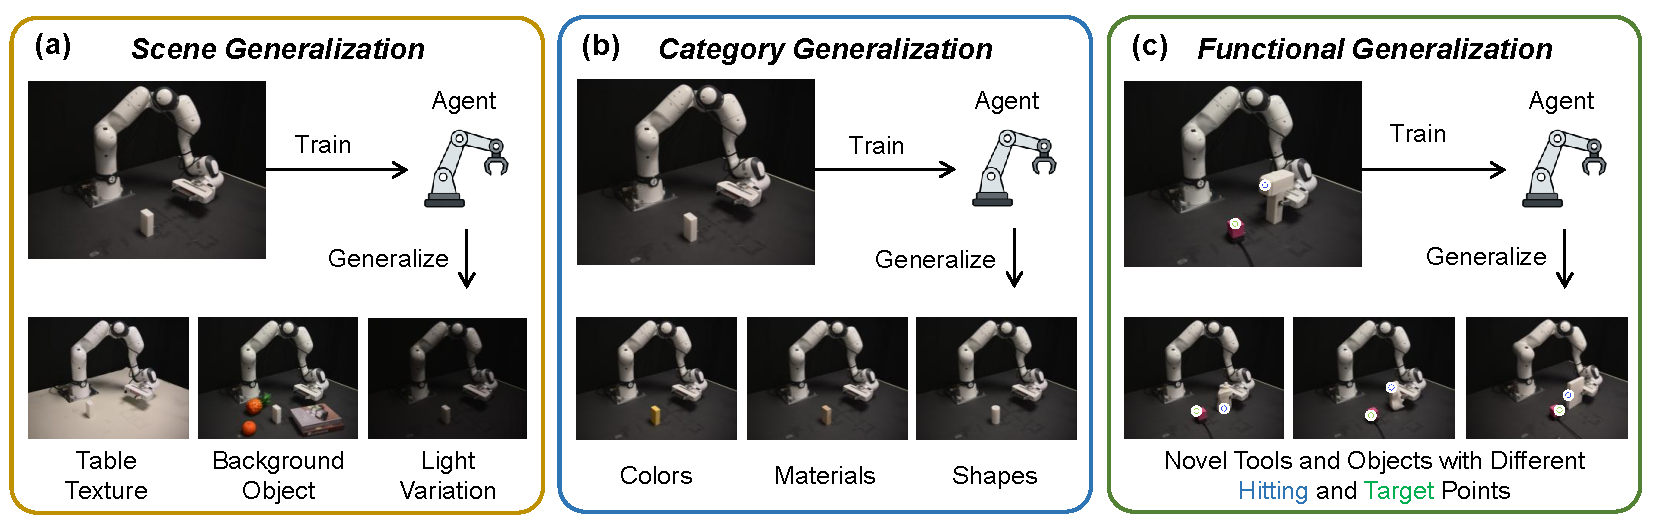
\includegraphics[width=1.0\linewidth]{figures/teaser_v2.pdf}
    \caption{
    \textbf{Comparison between functional generalization and existing generalization settings.}
    (a) Scene generalization evaluates robustness to visual variations.
    (b) Category generalization tests transfer across objects with diverse properties.
    (c) Functional generalization requires using unseen tools to accomplish the same function.
    % (d) The functional intent of hitting.
    }
    \label{fig:functional_generalization}
\end{figure}
Functional generalization is fundamentally harder than conventional generalization. As illustrated in Fig.~\ref{fig:functional_generalization}, scene- and category-level generalization only require tolerating visual variations while the underlying motion stays the same~\cite{goyal2023rvt, shridhar2023perceiver, shridhar2022cliport, nair2023r3m}. Functional generalization, by contrast, demands that the motion itself change: striking a target with a novel tool requires locating its contact region, aligning it, and producing an appropriate motion, even when the tool's shape and trajectory differ entirely from training. The core difficulty is a fundamental mismatch: functionally equivalent tools share recognizable structure in visual space, but this similarity does not transfer to action space, where each tool demands an entirely different motor pattern.


Bridging this perception-to-action gap requires an intermediate representation that carries functional intent across tools, satisfying two competing demands: expressive enough to capture where to make contact and how to move onto the target, yet grounded enough to be predicted from action-free observations without overfitting to tool-specific appearance. Dense representations like raw video entangle function-relevant cues with tool-specific appearance, while overly sparse ones discard the geometric and temporal structure needed for action. This trade-off raises the central question of our work: \textit{which representation best transfers functional intent from perception to action?}

To answer this question, we systematically evaluate intermediate representations 
including affordance images, human video prompts, and 2D keypoint trajectories, 
finding that keypoint trajectories best balance functional expressiveness and 
action groundability: they capture function-relevant contact and motion structure 
while discarding tool-specific appearance that causes overfitting. Building on 
this, we propose \textbf{F}uncti\textbf{O}nal \textbf{R}easoning and 
\textbf{G}rounded \textbf{E}xecution (\algoname{}), a two-stage policy that 
decouples functional reasoning from action execution: it first predicts 
generalizable keypoint trajectories for unseen tools from large-scale action-free 
data, then grounds these functional plans into executable robot actions using a 
small set of action-labeled demonstrations. We further introduce a seven-tool 
hitting-function benchmark, where \algoname{} consistently outperforms 
state-of-the-art methods on unseen tools in both simulation and the real world, 
achieving over $2\times$ improvement in average success rate. In summary, our 
contributions are threefold:
\begin{itemize}[leftmargin=*]
    \item We formalize \textit{functional generalization} in robotic tool-use 
    and identify the perception-to-action gap as its core difficulty.
    \item We find that 2D keypoint trajectories best balance functional 
    expressiveness and action groundability, and propose \algoname{}, a two-stage 
    policy that predicts generalizable keypoint trajectories from action-free data 
    and grounds them into robot actions with limited demonstrations.

    \item Through extensive simulation experiments across seven tools and real-world 
    validation, we demonstrate that \algoname{} consistently outperforms 
    state-of-the-art methods on unseen tools, achieving over $2\times$ improvement in average success rate.

\end{itemize}

% Intuitively, a straightforward method to address this problem is to expose agents to diverse tool-use demonstrations, allowing them to observe how different tools interact with the target over time. However, this strategy faces two key challenges. First, collecting large-scale action-labeled robotic data across diverse tools is time-consuming and labor-intensive, especially for contact-rich tool-use tasks. Additionally, direct visual-to-action learning compresses dense, semantics-rich observations into sparse motor commands, causing function-relevant structures to collapse into tool-specific action patterns. Consequently, the agents tend to overlook transferable cues, such as aligning hitting regions with the same target point, and fail on novel tools. These challenges necessitate a framework that decouples functional intent reasoning from action execution, enabling agents to extract transferable tool-use abstractions and ground them into precise low-level control.

% \lw{
% Bridging this gap requires an intermediate representation that carries the shared affordance from perception into action. 
% Such a representation must satisfy two competing demands. 
% On one hand, it should be \textit{expressive} enough to preserve the function-relevant structure shared across tools, namely, where to make contact and how to bring it onto the target. 
% On the other hand, it should be \textit{groundable}: predictable from action-free observations and decodable into precise actions, without smuggling in tool-specific appearance that the policy would simply overfit. 
% These demands are in tension. 
% Dense representations such as raw video preserve rich detail but entangle function-relevant cues with tool-specific appearance, while overly sparse representations discard the temporal and geometric structure needed to act. 
% This trade-off raises the central question of our work: \textit{which representation best carries affordance similarity from perception to action?}}


% Bridging this gap requires an intermediate representation that carries the shared affordance from perception into action. 
% Such a representation must satisfy two competing demands. 
% On one hand, it should be \textit{expressive} enough to preserve the function-relevant structure shared across tools, namely, where to make contact and how to bring it onto the target. 
% On the other hand, it should be \textit{groundable}: predictable from action-free observations and decodable into precise actions, without smuggling in tool-specific appearance that the policy would simply overfit. 
% These demands are in tension. 
% Dense representations such as raw video preserve rich detail but entangle function-relevant cues with tool-specific appearance, while overly sparse representations discard the temporal and geometric structure needed to act. 
% This trade-off raises the central question of our work: \textit{which representation best carries affordance similarity from perception to action?}


% When humans perform a task such as hitting a nail with an alternative tool, we typically reason about the functional interaction before execution by imagining how the tool may interact with the target, either as a future visual scene or as a possible motion trajectory. Inspired by this process, we aim to explore a functional intermediate representation that bridges dense visual observations and sparse motor commands. An effective representation should be visually predictable from action-free observations, while remaining sufficiently structured to support action grounding. With such a representation, a high-level planner can predict function-relevant future states, and a low-level execution policy can translate them into precise robot actions. This formulation reduces the burden of learning functional intent purely from action-labeled robot data and alleviates the information collapse caused by direct visual-to-action learning.

% In this paper, we propose the Generalizable Functional Plan and Execution (\algoname{}) policy, a System-2/System-1 framework that decouples functional planning from action execution using a functional intermediate representation. We study several candidate representations, including affordance images, human video prompts, and 2D keypoint trajectories, and find that 2D keypoint trajectories provide the best trade-off between visual predictability and action groundability. Our \algoname{} policy therefore trains a System-2 planner to predict future keypoint trajectories as functional plans, and a System-1 execution policy to ground these plans into executable actions. To evaluate functional generalization, we further introduce a hitting-function benchmark across seven tools. Experiments in simulation and real-world settings show that the \algoname{} policy consistently outperforms other state-of-the-art methods on unseen tools.

% \lw{
% To answer this question, we propose \algoname{} (Generalization via Functional Trajectories), a policy built on 2D keypoint trajectories as the functional intermediate representation. 
% Among affordance images, human video prompts, and keypoint trajectories, we find that keypoint trajectories best balance affordance expressiveness and action groundability: they retain the contact point, target, and tool geometry that define the affordance, while discarding the tool-specific appearance that a policy tends to overfit. 
% \algoname{} first predicts future keypoint trajectories from large-scale action-free observations, and then grounds the predicted plan into precise actions using only a small set of action-labeled demonstrations, sidestepping the prohibitive cost of learning functional structure from robot data alone. 
% To evaluate functional generalization, we further introduce a hitting-function benchmark across seven tools, where \algoname{} consistently outperforms state-of-the-art methods on unseen tools in both simulation and the real world, achieving over $2\times$ improvement in average success rate.
% }


% To this end, we propose \textbf{F}uncti\textbf{O}nal \textbf{R}easoning and \textbf{G}rounded \textbf{E}xecution (\algoname{}), a policy built on 2D keypoint trajectories as the functional intermediate representation. 
% Among affordance images, human video prompts, and keypoint trajectories, we find that keypoint trajectories best balance affordance expressiveness and action groundability: they retain the contact point, target, and affordance-relevant tool geometry, while discarding the tool-specific appearance that a policy tends to overfit. 
% \algoname{} first predicts future keypoint trajectories from large-scale action-free data, and then grounds them into actions using a small set of action-labeled demonstrations, sidestepping the prohibitive cost of learning functional structure from robot data alone.
% To evaluate functional generalization, we further introduce a hitting-function benchmark across seven tools, where \algoname{} outperforms state-of-the-art methods on unseen tools in simulation and the real world, achieving over $2\times$ improvement in average success rate. In summary, our contributions are threefold:

% In summary, our contributions are threefold:
% \begin{itemize}[leftmargin=*]
%     \item We identify \textit{functional generalization} as a novel problem in tool-use manipulation, aiming to evaluate whether agents can transfer the same function across diverse and unseen tools.

%     \item \textbf{\algoname{}} policy is proposed as a System-2/System-1 framework that uses 2D keypoint trajectories to bridge functional planning and action execution.

%     \item A 7-tool hitting-function benchmark is developed, where simulation and real-world experiments show that \algoname{} consistently outperforms state-of-the-art methods on unseen tools.
% \end{itemize}

% \lw{
% In summary, our contributions are threefold:
% \begin{itemize}[leftmargin=*]
%     \item We identify \textit{functional generalization} in tool-use manipulation, accomplishing the same function with diverse and unseen tools, and frame its core difficulty as carrying tool affordance from perception to action.
%     \item We find that 2D keypoint trajectories best balance affordance expressiveness and action groundability, and propose \textbf{\algoname{}}, which predicts keypoint trajectories from action-free data and grounds them into actions with limited robot demonstrations.
%     \item We build a seven-tool hitting-function benchmark, where \algoname{} outperforms state-of-the-art methods on unseen tools in both simulation and the real world, with over $2\times$ improvement in average success rate.
% \end{itemize}
% }
% \begin{itemize}[leftmargin=*]
%     \item We identify \textit{functional generalization} in robotic tool-use, completing the same function with unseen tools, and frame its core difficulty as carrying tool affordance from perception to action.
%     \item We find that 2D keypoint trajectories best balance affordance expressiveness and action groundability, and propose \algoname{}, which predicts keypoint trajectories from action-free data and grounds them into actions with limited robotic demonstrations.
%     \item A 7-tool hitting-function benchmark is built, where \algoname{} outperforms state-of-the-art methods on unseen tools in simulation and the real world, with over $2\times$ improvement in success rate.
% \end{itemize}


%===============================================================================

\section{Related Works}
\label{sec:related_works}

\paragraph{Generalization Problems in Robotic Manipulation.}
Generalization has been a central problem in robotic manipulation, and existing studies mainly evaluate it from three perspectives: scene-level, category-level, and cross-embodiment generalization.
Scene-level generalization focuses on whether a policy can remain robust when the surrounding visual or physical contexts vary, such as changes in object layouts, lighting conditions, or camera viewpoints~\cite{goyal2023rvt, shridhar2023perceiver, shridhar2022cliport, nair2023r3m}. 
Furthermore, category-level generalization studies whether robots can transfer manipulation skills to unseen objects that belong to the same semantic category while differing in geometry, size, or texture~\cite{gao2021kpam, mo2021where2act, geng2023gapartnet}.
More recently, cross-embodiment generalization has attracted increasing attention, which aims to train a unified policy that can transfer across different robot platforms, such as robotic arms and humanoids~\cite{o2024open, team2024octo, intelligence2025pi}.
In this work, we go beyond generalization over visual appearance and robot embodiment and focus on \textit{functional generalization}, in which an agent is required to accomplish the same function using diverse, unseen tools.


\paragraph{Improving Generalization in Robot Policy Learning.}
To improve manipulation generalization, the most straightforward way is scaling up action-labeled robotic data and training policies end-to-end~\cite{zitkovich2023rt, o2024open, team2024octo, khazatsky2024droid}. 
However, collecting large-scale robotic data is time-consuming and labor-intensive, especially for complicated tool-use manipulations. 
Reducing the dependence on action labels, some works learn transferable motion priors from large-scale action-free video data~\cite{nair2023r3m, wang2023mimicplay, wu2024unleashing,ma2026dit4dit, pai2025mimic, an2026feedback, hou2026world}. 
For example, MimicPlay~\cite{wang2023mimicplay} learns high-level latent plans from human play videos and grounds them into robot actions with a low-level visuomotor policy. 
Although videos contain rich motion and interaction cues, dense future frames do not explicitly reveal a compact abstraction of function-relevant intent. As a result, effectively learning functional priors from videos often requires extremely extensive pretraining.
Another line of work improves action grounding with more structured intermediate representations, such as interaction heatmaps~\cite{mo2021where2act, bahl2023affordances, wu2025afforddp, li2026compassad}, object-centric representations~\cite{zhulearning, chen2025tool, chapin2025object}, or keypoint trajectories~\cite{gao2021kpam, huang2025rekep, turpin2021gift, wen2023any}. 
For instance, ATM~\cite{wen2023any} predicts future trajectories of arbitrary points from video and uses them to guide a low-level policy for action generation. 
However, these methods mainly focus on standard manipulation tasks, such as object pick-up, while overlooking tool-use scenarios that require capturing more abstract functional intent, which are systematically investigated in our work. 
% through the lens of different intermediate representations.
% However, these methods mainly focus on standard manipulation tasks, such as object pick up, while overlooking tool-use scenarios that require understanding more abstract functional intent. 
% In this work, we systematically investigate the effect of different intermediate representations on functional generalization and identify that keypoint trajectories provide the best trade-off between visual predictability and action groundability.

%\paragraph{Intermediate Representations for Tool-use Manipulation.}
% Instead of directly predicting low-level actions from raw observations, many manipulation methods introduce intermediate representations to provide more structured guidance. Affordance-based methods identify task-relevant object regions for interaction, while keypoint-based methods represent objects or tools using sparse semantic points to support category-level manipulation and action grounding. Other works use human videos or predicted future observations as high-level plans, which can capture task intent before execution. These intermediate signals improve interpretability and transferability, but they often differ in visual predictability and action groundability. For contact-rich tool-use tasks, an effective representation should not only capture where the functional interaction occurs, but also describe how the tool should move over time. In this work, we systematically study several candidate representations, including affordance images, human video prompts, and 2D keypoint trajectories, and show that keypoint trajectories provide a better trade-off between functional planning and executable action grounding.

% Improving the generalization capability of robotic policies is a central challenge for deploying robots in open-world environments. Existing methods mainly address this problem from three perspectives.

% \paragraph{Scaling up Robotic Data.}
% One direct way to improve generalizable planning is to scale up robotic demonstrations and train policy models end-to-end to predict actions from observations~\cite{}. For example, Open X-Embodiment~\cite{} aggregates large-scale robot trajectories from many laboratories and enables RT-X to learn transferable skills across tasks and embodiments. Similarly, Octo~\cite{} trains a generalist policy on heterogeneous robot datasets and shows strong multi-task manipulation ability. However, collecting large-scale robot data is extremely labor-intensive and time-consuming, and the resulting policies may still lack explicit functional abstraction beyond the demonstrated objects and scenes.

% \paragraph{Pretraining on Human Videos.}
% Another direction is to pretrain policy models on action-free human videos to learn motion priors, and then transfer these priors to robot action generation through fine-tuning on a small amount of robotic demonstrations. For instance, R3M~\cite{} learns reusable visual representations from large-scale human videos and transfers them to downstream robot manipulation tasks. MimicPlay~\cite{} further extracts high-level plans from human play videos and grounds them with a low-level robot policy. However, without explicit action or physical supervision, it is difficult for models to learn the precise dynamics required for motor control, which may require extremely large-scale video pretraining.

% \paragraph{Exploiting Foundation Models.}
% Another stream of works~\cite{} uses pretrained foundation models to extract generalizable affordance or planning signals, which serve as intermediate bridges between seen and unseen demonstrations. For example, RT-H~\cite{} leverages vision-language reasoning to predict action hierarchies, allowing high-level semantic plans to guide low-level robot execution. Large Video Planner further takes a video foundation model as a high-level planner to predict future visual plans, which are then grounded into robot actions by a low-level policy. However, using foundation models during inference can introduce significant latency, and the final policy performance is strongly limited by the accuracy of the predicted intermediate signals.

% \paragraph{Summary.}
% Beyond data-centric strategies, recent methods~\cite{} exploit pretrained foundation models to extract generalizable affordance or planning signals, which serve as intermediate bridges between seen and unseen demonstrations. The goal is to enable a policy to transfer the same functional behavior, such as hitting, to novel tools with different shapes, materials, and interaction regions. To this end, we propose an efficient System-2 plus System-1 architecture, where System-2 predicts generalizable intermediate functional plans and System-1 grounds these plans into executable robot actions. This design aims to bridge high-level functional reasoning and low-level action execution, thereby improving policy generalization beyond object-specific imitation.


%===============================================================================

\begin{figure}[ht]
    \centering
    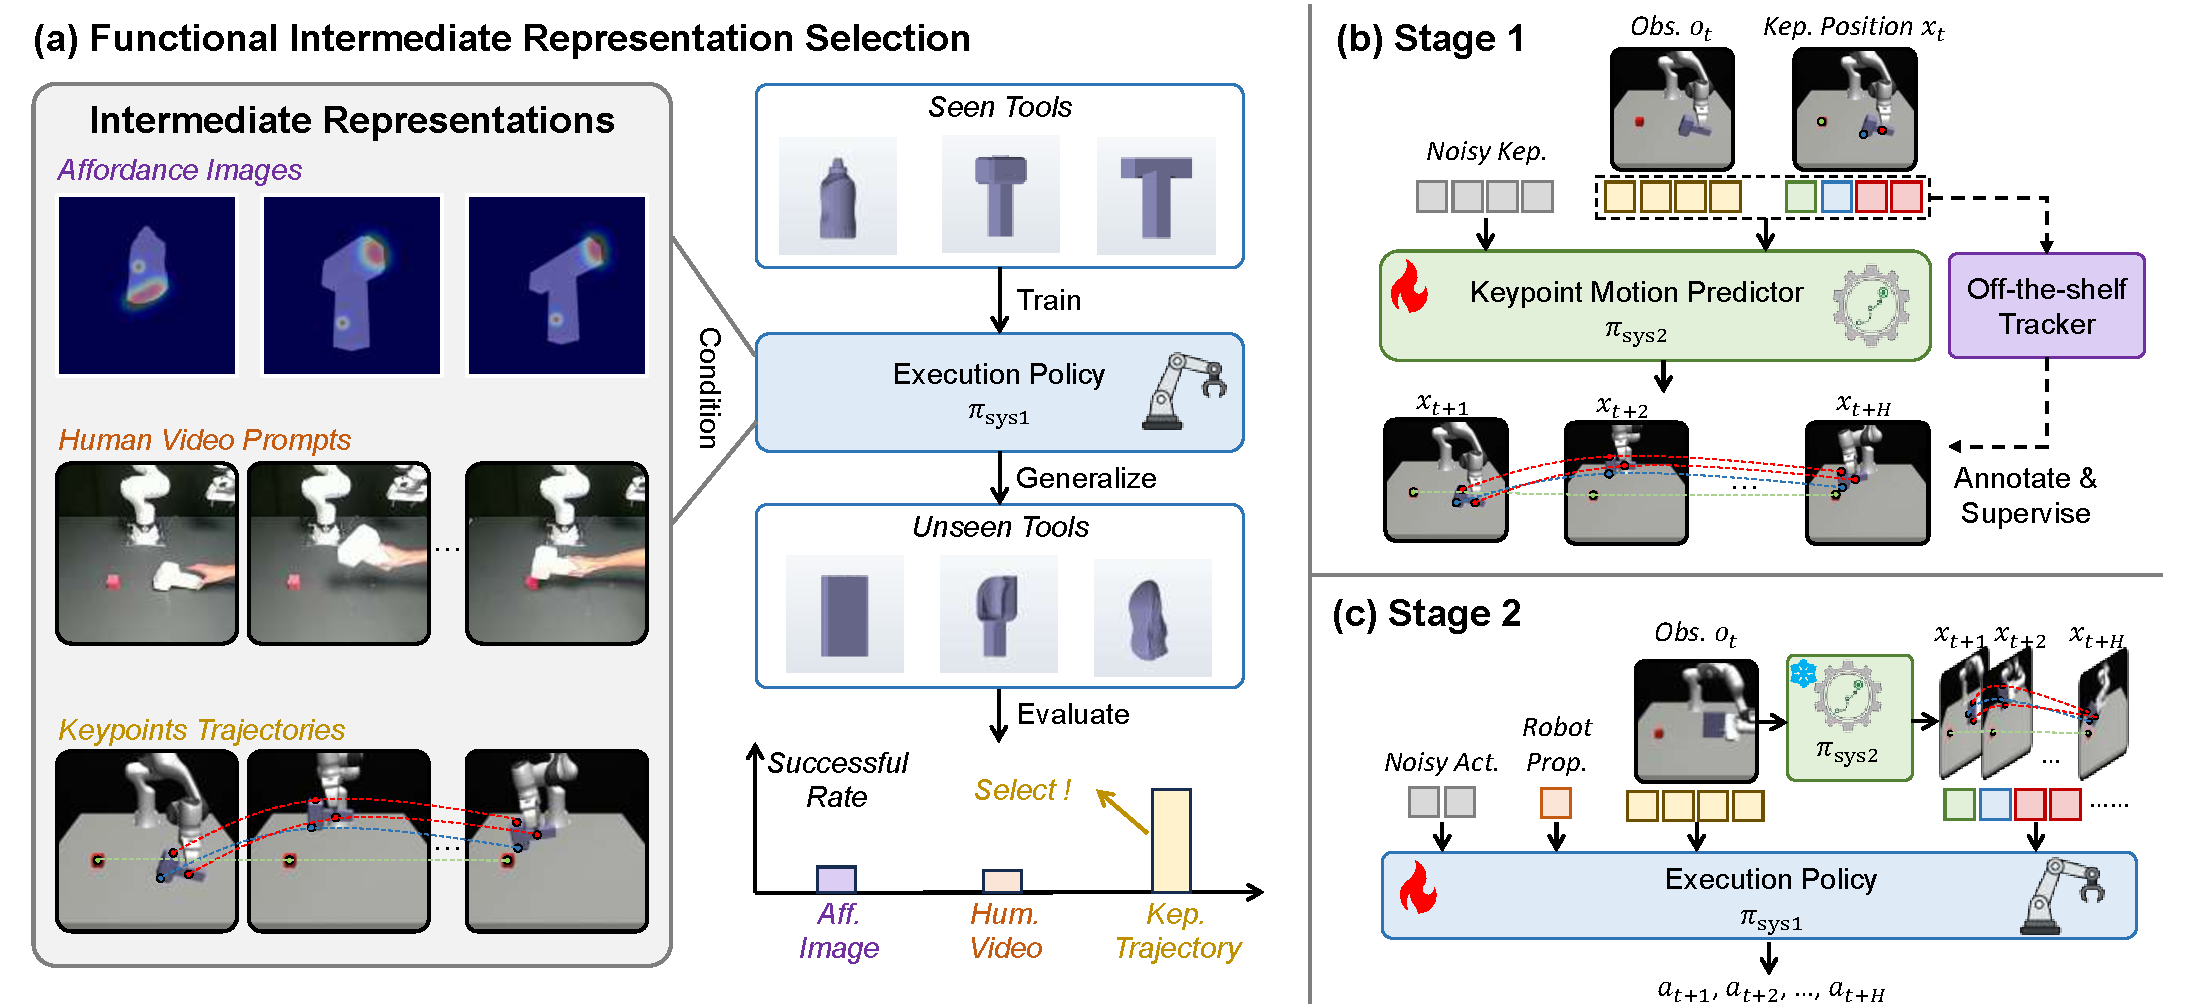
\includegraphics[width=1.0\linewidth]{figures/main_pipeline.pdf}
    \caption{
    \textbf{Overview of the \algoname{}.} (a) Evaluation and selection of functional intermediate representations. (b) In Stage 1, the System-2 planner learns to predict future keypoint-based functional plans from action-free observations. (c) In Stage 2, the System-1 execution policy grounds the predicted functional plans into executable robot actions.
    }
    \label{fig:functional_generalization_pipeline}
\end{figure}

\section{Methods}
\label{sec:method}

% \subsection{Problem Formulation}
% Our Generalizable Function Plan and Execution (\algoname{}) policy follows a human-inspired dual-system architecture. Given the visual observation $o_{t}$ at time step $t$, the System-2 policy $\pi_{\mathrm{sys}\text{-}2}$ predicts a high-level functional plan, denoted as $x_{t:t+H} = \pi_{\mathrm{sys}2}(o_{t})$, where $x_{t:t+H}$ serves as a trade-off representation over a future horizon $H$. This representation is more structured than dense visual features and more abstract than low-level motor commands, making it suitable for bridging functional planning and action grounding. The System-1 policy $\pi_{\mathrm{sys}1}$ then grounds this plan into executable actions, denoted as ${a}_{t:t+H} = \pi_{\mathrm{sys}\text{-}1}(o_{t}, q_{t}, {x}_{t:t+H})$, by conditioning on the visual observation ${o}_{t}$, the robot proprioceptive state $q_{t}$, and the predicted trade-off representation $x_{t:t+H}$.

% To achieve this goal, we assume access to two types of training data. The first is a large-scale action-free dataset $\mathcal{D}_{U} = \{(o^{i}_{t}, x^{i}_{t:t+H})\}_{i=1}^{N_{U}}$, where each sample contains a visual observation and its corresponding trade-off representation, without requiring robot action labels. The second is a smaller action-labeled dataset $\mathcal{D}_{L} = \{(o^{i}_{t}, q^{i}_{t}, a^{i}_{t:t+H})\}_{i=1}^{N_{L}}$, where each sample provides the visual observation, robot proprioceptive state, and action trajectory label. We first pretrain the System-2 policy $\pi_{\mathrm{sys}\text{-}2}$ on $\mathcal{D}_{U}$ to learn function-relevant planning from action-free data. We then integrate the pretrained System-2 module with the System-1 execution policy and finetune the overall \algoname{} policy on $\mathcal{D}_{L}$, enabling the model to translate high-level functional plans into executable robot actions.

% Our Generalizable Function Plan and Execution (\algoname{}) policy follows a human-inspired dual-system architecture. Assume that two datasets are accessible: a large-scale action-free dataset $\mathcal{D}_{U}=\{(\mathbf{O}^{(i)}, \mathbf{X}^{(i)})\}_{i=1}^{N_U}$, where each sample contains a sequence of visual observations $\mathbf{O}^{(i)}=\{o_{t}^{(i)}\}_{t=1}^{T}$ and the corresponding trade-off representations $\mathbf{X}^{(i)}=\{x_{t}^{(i)}\}_{t=1}^{T}$; and a smaller action-labeled robotic dataset $\mathcal{D}_{L}=\{(\mathbf{O}^{(i)}, \mathbf{Q}^{(i)}, \mathbf{A}^{(i)})\}_{i=1}^{N_L}$, where $\mathbf{Q}^{(i)}=\{q_{t}^{(i)}\}_{t=1}^{T}$ denotes the robot proprioceptive states and $\mathbf{A}^{(i)}=\{a_{t}^{(i)}\}_{t=1}^{T}$ denotes the action labels. Our objective is to first learn a System-2 policy $\pi_{\mathrm{sys}2}$ from $\mathcal{D}_{U}$, which predicts a future function-relevant plan from the current visual observation and trade-off representation: $x_{t:t+H}=\pi_{\mathrm{sys}2}(o_t,x_t)$. We then finetune both $\pi_{\mathrm{sys}2}$ and the System-1 policy $\pi_{\mathrm{sys}1}$ on $\mathcal{D}_{L}$, so that the predicted functional plan can be grounded into executable actions: $a_{t:t+H}=\pi_{\mathrm{sys}1}(o_t,q_t,\pi_{\mathrm{sys}2}(o_t,x_t))$. At test time, for an unseen tool-use sample $(\mathbf{O}^{*}, \mathbf{Q}^{*}, \mathbf{A}^{*}) \notin \mathcal{D}_{L}$, \algoname{} generates the action trajectory $a_{t:t+H}^{*}=\pi_{\mathrm{sys}1}(o_t^{*},q_t^{*},\pi_{\mathrm{sys}2}(o_t^{*},x_t^{*}))$ to accomplish the hitting function.

% Our Generalizable Function Plan and Execution (\algoname{}) policy follows a human-inspired dual-system architecture. Assume that two datasets are accessible: a large-scale action-free dataset $\mathcal{D}_{U}=\{(\mathbf{O}^{(i)}, \mathbf{X}^{(i)})\}_{i=1}^{N_U}$, where each sample contains a sequence of visual observations $\mathbf{O}^{(i)}=\{o_{t}^{(i)}\}_{t=1}^{T}$ and the corresponding trade-off representations $\mathbf{X}^{(i)}=\{x_{t}^{(i)}\}_{t=1}^{T}$; and a smaller action-labeled robotic dataset $\mathcal{D}_{L}=\{(\mathbf{O}^{(i)}, \mathbf{X}^{(i)}, \mathbf{Q}^{(i)}, \mathbf{A}^{(i)})\}_{i=1}^{N_L}$, where $\mathbf{Q}^{(i)}=\{q_{t}^{(i)}\}_{t=1}^{T}$ denotes the robot proprioceptive states and $\mathbf{A}^{(i)}=\{a_{t}^{(i)}\}_{t=1}^{T}$ denotes the action labels. Our objective is to learn a System-2 policy $\pi_{\mathrm{sys}2}$ from $\mathcal{D}_{U}$, which predicts a future function-relevant plan from the current visual observation and trade-off representation: $x_{t:t+H}=\pi_{\mathrm{sys}2}(o_t,x_t)$. We then finetune both $\pi_{\mathrm{sys}2}$ and the System-1 policy $\pi_{\mathrm{sys}1}$ on $\mathcal{D}_{L}$, so that the predicted functional plan can be grounded into executable actions: $a_{t:t+H}=\pi_{\mathrm{sys}1}(o_t,q_t,\pi_{\mathrm{sys}2}(o_t,x_t))$. At test time, for an unseen tool-use sample $(\mathbf{O}^{*}, \mathbf{Q}^{*}, \mathbf{A}^{*}) \notin \mathcal{D}_{L}$, \algoname{} policy is expected to generate the action trajectory $a_{t:t+H}^{*}=\pi_{\mathrm{sys}1}(o_t^{*},q_t^{*},\pi_{\mathrm{sys}2}(o_t^{*},x_t^{*}))$ to accomplish the hitting function.

% \subsection{Problem Formulation}
% Our Generalizable Functional Plan and Execution (\algoname{}) policy follows a human-inspired dual-system architecture, where a high-level System-2 planner predicts function-relevant future states and a low-level System-1 policy grounds them into executable robot actions. 
% We assume that two types of datasets are accessible. 
% The first is a large-scale action-free dataset 
% $\mathcal{D}_{U}=\{(\mathbf{O}^{(i)}, \mathbf{X}^{(i)})\}_{i=1}^{N_U}$, 
% where $\mathbf{O}^{(i)}=\{o_t^{(i)}\}_{t=1}^{T}$ denotes a sequence of visual observations, and 
% $\mathbf{X}^{(i)}=\{x_t^{(i)}\}_{t=1}^{T}$ denotes the corresponding functional intermediate representations which describe functional-relevant future states. 
% % These representations describe task-relevant functional states, such as future keypoint trajectories, without requiring robot action labels. 
% The second is a smaller action-labeled robotic dataset 
% $\mathcal{D}_{L}=\{(\mathbf{O}^{(i)}, \mathbf{X}^{(i)}, \mathbf{Q}^{(i)}, \mathbf{A}^{(i)})\}_{i=1}^{N_L}$, 
% where $\mathbf{Q}^{(i)}=\{q_t^{(i)}\}_{t=1}^{T}$ means robot proprioceptive states and 
% $\mathbf{A}^{(i)}=\{a_t^{(i)}\}_{t=1}^{T}$ represents ground-truth actions.

% Given observation $o_t$ and functional representation $x_t$ at time-step $t$, the System-2 planner 
% $\pi_{\mathrm{sys2}}$ predicts a future functional plan over horizon $H$:
% \begin{equation}
%     \hat{\mathbf{X}}_{t:t+H}
%     =
%     \pi_{\mathrm{sys2}}(o_t, x_t).
% \end{equation}
% The System-1 execution policy $\pi_{\mathrm{sys1}}$ then grounds this predicted plan into an action trajectory conditioned on the current observation and robot state:
% \begin{equation}
%     \hat{\mathbf{A}}_{t:t+H}
%     =
%     \pi_{\mathrm{sys1}}(o_t, q_t, \hat{\mathbf{X}}_{t:t+H}).
% \end{equation}
% % Therefore, \algoname{} first learns functional planning from action-free data and then learns action grounding from limited action-labeled demonstrations. 
% % At test time, given an unseen tool, \algoname{} predicts a future functional plan and grounds it into robot actions to accomplish the same hitting function with the novel tool.
% Consequently, the objective of \algoname{} is to learn a functional planner from action-free data and an execution policy from limited action-labeled data, such that the predicted functional plans can be grounded into executable robot actions. 
% At test time, given an unseen tool, the \algoname{} policy predicts a future functional plan and translates it into actions to accomplish the same hitting function with the novel tool.






\subsection{Problem Formulation}
% Our Functional Reasoning and Grounded Execution (\algoname{}) policy follows a dual-system architecture for functional generalization in tool-use manipulation. \lw{introduce the problem first, something like MDP}
% Given a task function, such as hitting a target object, the goal is to learn a policy that can accomplish the same function with novel tools whose visual appearances and geometries differ from those observed during training.

% We assume that two types of datasets are available. 
% The first is a large-scale action-free dataset 
% $\mathcal{D}_{U}=\{(\mathbf{O}^{(i)}, \mathbf{X}^{(i)})\}_{i=1}^{N_U}$, 
% where $\mathbf{O}^{(i)}=\{\mathbf{o}^{(i)}_t\}_{t=1}^{T}$ denotes a sequence of visual observations, and 
% $\mathbf{X}^{(i)}=\{\mathbf{x}^{(i)}_t\}_{t=1}^{T}$ denotes the corresponding functional intermediate representations that describe function-relevant future states. 
% The second is a smaller action-labeled robotic dataset 
% $\mathcal{D}_{L}=\{(\mathbf{O}^{(i)}, \mathbf{X}^{(i)}, \mathbf{Q}^{(i)}, \mathbf{A}^{(i)})\}_{i=1}^{N_L}$, 
% where $\mathbf{Q}^{(i)}=\{\mathbf{q}^{(i)}_t\}_{t=1}^{T}$ represents robot proprioceptive states and 
% $\mathbf{A}^{(i)}=\{\mathbf{a}^{(i)}_t\}_{t=1}^{T}$ denotes ground-truth robot actions.

% The objective of \algoname{} is decoupled into two sub-problems.
% First, a System-2 planner learns from action-free data to predict a functional plan in the space of intermediate representations. 
% Second, a System-1 execution policy grounds the predicted functional plan into executable robot actions via finetuning on action-labeled data. 
% This decomposition allows \algoname{} to leverage scalable action-free data for functional reasoning, while using limited robotic demonstrations for action grounding.

% \lw{
% We formulate functional generalization in tool-use manipulation as a Markov Decision Process (MDP), where the state $\mathbf{s}_t$ consists of the visual observation $\mathbf{o}_t$ and the robot proprioceptive state $\mathbf{q}_t$, and the action $\mathbf{a}_t$ is a motor command. A task function (e.g., hitting a target) is associated with a set of seen tools $\mathcal{T}_{\text{seen}}$ used for training and a disjoint set of unseen tools $\mathcal{T}_{\text{unseen}}$ used for evaluation, where the function stays fixed but the tool, its appearance, and its required motion all change. Two types of data are available for learning. The first is a large-scale action-free dataset $\mathcal{D}_{U}=\{(\mathbf{O}^{(i)}, \mathbf{X}^{(i)})\}_{i=1}^{N_U}$, consisting of visual observations $\mathbf{O}^{(i)}=\{\mathbf{o}^{(i)}_t\}_{t=1}^{T}$ and corresponding functional intermediate representations $\mathbf{X}^{(i)}=\{\mathbf{x}^{(i)}_t\}_{t=1}^{T}$ (e.g., 2D keypoint trajectories from an off-the-shelf tracker), which is abundant since it requires no robot labels. The second is a smaller action-labeled robotic dataset $\mathcal{D}_{L}=\{(\mathbf{O}^{(i)}, \mathbf{X}^{(i)}, \mathbf{Q}^{(i)}, \mathbf{A}^{(i)})\}_{i=1}^{N_L}$, which additionally provides proprioceptive states $\mathbf{Q}^{(i)}$ and ground-truth actions $\mathbf{A}^{(i)}$ but is costly to collect, so $|\mathcal{D}_L| \ll |\mathcal{D}_U|$. This data asymmetry, together with the affordance-to-action gap discussed in Sec.~\ref{sec:intro}, motivates a two-stage decomposition: \algoname{} learns a future-state predictor on $\mathcal{D}_U$ that forecasts the functional intermediate representation from observations, and an execution policy on $\mathcal{D}_L$ that grounds the predicted representation into robot actions.
% }

We formulate functional generalization in tool-use manipulation as a Markov Decision Process (MDP), where the state $\mathbf{s}_t$ consists of the visual observation $\mathbf{o}_t$, the proprioceptive state $\mathbf{q}_t$, and optionally a functional intermediate representation $\mathbf{x}_t$ (e.g., affordance images, human video prompts, or keypoint trajectories) that carries function-relevant cues bridging perception and action, and the action $\mathbf{a}_t$ is the motor command. A task function (e.g., hitting a target) is defined over seen tools $\mathcal{T}_{\text{seen}}$ for training and disjoint unseen tools $\mathcal{T}_{\text{unseen}}$ for evaluation, where the function stays fixed but the tool, its appearance, and the required contact positions and motions all change.


%We formulate functional generalization in tool-use manipulation as a Markov Decision Process (MDP), where the state $\mathbf{s}_t$ consists of the visual observation $\mathbf{o}_t$, the robot proprioceptive state $\mathbf{q}_t$, and optionally a functional intermediate representation $\mathbf{x}_t$, while action $\mathbf{a}_t$ denotes the motor command.
%The functional intermediate representation is expected to carry function-relevant cues that bridge perception and action, such as contact regions, target locations, or motion patterns. It can be instantiated in various forms, e.g., affordance images, human video prompts, or keypoint trajectories.
%A task function (e.g., hitting a target) is associated with a set of seen tools $\mathcal{T}_{\text{seen}}$ used for training and a disjoint set of unseen tools $\mathcal{T}_{\text{unseen}}$ used for evaluation, where the function stays fixed but the tool, its appearance, and its required hitting and target positions as well as motions all change. 

Two types of data are available for learning. The first is a large-scale action-free dataset $\mathcal{D}_{U}=\{(\mathbf{O}^{(i)}, \mathbf{X}^{(i)})\}_{i=1}^{N_U}$, consisting of visual observations $\mathbf{O}^{(i)}=\{\mathbf{o}^{(i)}_t\}_{t=1}^{T}$ and corresponding functional intermediate representations $\mathbf{X}^{(i)}=\{\mathbf{x}^{(i)}_t\}_{t=1}^{T}$, which is abundant since it requires no robot labels.
The second is a smaller action-labeled robotic dataset $\mathcal{D}_{L}=\{(\mathbf{O}^{(i)}, \mathbf{X}^{(i)}, \mathbf{Q}^{(i)}, \mathbf{A}^{(i)})\}_{i=1}^{N_L}$, which additionally provides proprioceptive states $\mathbf{Q}^{(i)}$ and ground-truth actions $\mathbf{A}^{(i)}$ but is costly to collect, so $|\mathcal{D}_L| \ll |\mathcal{D}_U|$. This data asymmetry, together with the perception-to-action gap discussed in Sec.~\ref{sec:intro}, motivates a two-stage decomposition: 
\begin{equation}
\underbrace{
\pi_{\mathrm{FORGE}}(
\mathbf{a}_{t:t+H} \mid \mathbf{o}_{t}, \mathbf{q}_{t}, \mathbf{x}_{t}
)
}_{\text{FORGE}}=
\underbrace{
\pi_{\mathrm{sys2}}(
\hat{\mathbf{X}}_{t:t+H} \mid \mathbf{o}_{t}, \mathbf{x}_{t}
)
}_{\text{functional reasoning}}
\underbrace{
\pi_{\mathrm{sys1}}(
\mathbf{a}_{t:t+H} \mid \mathbf{o}_{t}, \mathbf{q}_{t}, \hat{\mathbf{X}}_{t:t+H}
)
}_{\text{grounded execution}} .
\label{eq:forge_decomposition}
\end{equation}
% \algoname{} learns a future-state predictor on $\mathcal{D}_U$ that forecasts the functional intermediate representation from observations, and an execution policy on $\mathcal{D}_L$ that grounds the predicted representation into robot actions.
\algoname{} learns a future predictor on $\mathcal{D}_U$ for forecasting functional intermediate representations from observations, and an execution policy on $\mathcal{D}_L$ for grounding predicted representations into actions.

%(e.g., 2D keypoint trajectories from an off-the-shelf tracker),  






% \subsection{Selection of Trade-off Representations}
% The core component of the \algoname{} policy is the selection of trade-off representations $\mathbf{X}^{(i)}=\{x_{t}^{(i)}\}_{t=1}^{T}$ for each sample. Ideally, $\mathbf{X}^{(i)}$ should serve as an intermediate abstraction between high-level visual features and low-level action commands, balancing visual learnability and control generalization.

% To this end, we adopt a simple yet effective empirical strategy for selecting $\mathbf{X}^{(i)}$. As shown in Fig.~\ref{fig:functional_generalization_pipeline}(a), for each sample in $\mathcal{D}_{L}$, we collect a set of visually grounded intermediate representations, including affordance images $I_{\mathrm{aff}}$, human video prompts $\mathbf{V}_{\mathrm{hum}} = \{I^t_{\mathrm{hum}}\}_{t=1}^{T}$, and keypoint trajectories $\mathbf{P}=\{\mathbf{p}_{t}\}_{t=1}^{T},\ \mathbf{p}_{t}=\{\mathbf{p}_{t}^{k}\}_{k=1}^{K}$. \textcolor{red}{Please refer to the appendix for more details of our hitting benchmarks.} %and directly evaluate their generalization ability on unseen tools. 

% \paragraph{Affordance Image.}
% For each tool, we manually annotate its function-relevant hitting region and grasp point, which together form an affordance image. The affordance image is encoded by an image encoder $E_{\mathrm{aff}}$~\cite{} and serves as a consistent trade-off representation across all time steps:
% \begin{equation}
%     x_{t}^{(i)} = E_{\mathrm{aff}}\left(I_{\mathrm{aff}}^{(i)}\right) \in \mathbb{R}^{d},
%     \quad t=1,\ldots,T ,
% \end{equation}
% where $I_{\mathrm{aff}}^{(i)}$ denotes the annotated affordance image of the $i$-th tool-use sample, and $d$ is the feature dimension.

% \paragraph{Human Video Prompt.}
% Additionally, we record a human demonstration video of using each tool to perform the hitting function. The video prompt captures the function-relevant motion pattern required by hitting, including the alignment between the hitting region and the target point, as well as the subsequent downward striking motion. Formally, we encode the human video prompt using the WAN 2.1 video encoder $E_{\mathrm{vid}}$~\cite{} and apply average pooling to obtain the sequence-level representation, which is shared across all time steps as the trade-off representations:
% \begin{equation}
%     x_{t}^{(i)} =
%     \mathrm{AvgPool}
%     \left(
%     E_{\mathrm{vid}}\left(\mathbf{V}_{\mathrm{hum}}^{(i)}\right)
%     \right)
%     \in \mathbb{R}^{d},
%     \quad t=1,\ldots,T ,
% \end{equation}
% where $V_{\mathrm{hum}}^{(i)}$ denotes the human video prompt of the $i$-th tool-use sample.

% \paragraph{Keypoint Trajectories.}
% We further consider keypoint trajectories as dynamic trade-off representations. Specifically, our keypoints include the hitting point, the target point, and uniformly sampled tool keypoints, resulting in $K$ keypoints for each frame. Based on the initial positions, we use CoTracker~\cite{} to obtain a keypoint trajectory $\mathbf{P}^{(i)}=\{\mathbf{p}_{t}^{(i)}\}_{t=1}^{T}$, where $\mathbf{p}_{t}^{(i)}=\{\mathbf{p}_{t}^{(i),k}\}_{k=1}^{K}$ denotes the set of $K$ keypoints at time step $t$. For each time step, we flatten the keypoints and project them into a dynamic trade-off representation using a keypoint encoder $E_{\mathrm{kp}}$:
% \begin{equation}
%     x_{t}^{(i)}
%     =
%     E_{\mathrm{kp}}
%     \left(
%     \mathrm{Flatten}
%     \left(
%     \mathbf{p}_{t}^{(i)}
%     \right)
%     \right)
%     \in \mathbb{R}^{d},
%     \quad t=1,\ldots,T ,
% \end{equation}


% Based on different trade-off representations, we train the System-1 policy $\pi_{\mathrm{sys}1}$ on the action-labeled dataset $\mathcal{D}_{L}$ with a conditional flow-matching objective. Given a ground-truth action chunk $a_{t:t+H}$, a Gaussian noise sample $\epsilon \sim \mathcal{N}(0,\mathbf{I})$, and an interpolation time $\tau \sim \mathcal{U}(0,1)$, we define the interpolated action trajectory as $a_{t:t+H}^{\tau}=\tau a_{t:t+H}+(1-\tau)\epsilon$. The System-1 policy learns a conditional velocity field $v_{\theta}$ by minimizing:
% \begin{equation}
%     \mathcal{L}_{\mathrm{fm}}
%     =
%     \mathbb{E}_{\tau,\epsilon,\mathcal{D}_{L}}
%     \left[
%     \left\|
%     v_{\theta}
%     \left(
%     a_{t:t+H}^{\tau},
%     \tau
%     \mid
%     o_t, q_t, x_{t:t+H}
%     \right)
%     -
%     \left(
%     a_{t:t+H}-\epsilon
%     \right)
%     \right\|_{2}^{2}
%     \right],
% \end{equation}

% Afterwards, we directly evaluate each variant on unseen tool samples $(\mathbf{O}^{*}, \mathbf{Q}^{*}, \mathbf{A}^{*}) \notin \mathcal{D}_{L}$. Specifically, given the corresponding annotated trade-off representation $\mathbf{X}^*$ for each unseen tool, the trained System-1 policy predicts the action trajectory $a^*_{t:t+H}=\pi_{\mathrm{sys1}}(o^*_t,q^*_t,x^*_{t:t+H})$ to control the unseen tools to complete the hitting function. We then compare the task success rates across different representations and identify keypoint trajectories $\mathbf{P}=\{\mathbf{p}_{t}\}_{t=1}^{T}$ as the most effective trade-off representations for bridging functional planning and action grounding.

% On the other hand, it should be \textit{groundable}: predictable from action-free observations and decodable into precise actions, without smuggling in tool-specific appearance that the policy would simply overfit. 
















% \subsection{Functional Intermediate Representations Selection}
% \label{Functional-Intermediate-Representations-Selection}
% \lw{make it more connected to the previous section} The core component of \algoname{} policy is the selection of functional intermediate representations $\mathbf{X}^{(i)}=\{x_t^{(i)}\}_{t=1}^{T}$. 
% As discussed in Sec.~\ref{sec:intro}, a desired representation should be visually predictable from action-free observations while remaining structured enough to be decoded into precise actions. 
% % This balance is critical for learning transferable functional plans and translating them into executable robot actions.

% To study this trade-off, as illustrated in Fig.~\ref{fig:functional_generalization_pipeline}~(a), we evaluate three representative functional intermediate representations from each action-labeled sample in $\mathcal{D}_{L}$, including the affordance image, human video prompt, and 2D keypoint trajectories.
% Particularly, affordance images provide static functional cues about the grasp point and contact regions. 
% Human video prompts illustrate dense visual demonstrations of how the tool should move to accomplish the hitting function. 
% 2D keypoint trajectories provide compact geometric motion cues by tracking the hitting point, the target, and sampled tool points over time. 
% Please refer to the appendix for details on how these representations are extracted. 
% These representations are encoded as the functional condition for the System-1 policy: 

% \textbf{Affordance Image.}~~
% % An affordance image provides a static description of function-relevant tool regions, including the grasp region and the hitting region. 
% Given an affordance image $I_{\mathrm{aff}}^{(i)}$, we encode it with an image encoder $E_{\mathrm{aff}}$~\cite{he2016deep} and use the resulting feature as a time-invariant condition: $x_t^{(i)}=E_{\mathrm{aff}}(I_{\mathrm{aff}}^{(i)})\in\mathbb{R}^{d}$.

% \textbf{Human Video Prompt.}~~
% %A human video prompt provides dense visual evidence of the functional interaction process, including target alignment and the subsequent striking motion. 
% Given a human demonstration video $V_{\mathrm{hum}}^{(i)}=\{I_{\mathrm{hum},t}^{(i)}\}_{t=1}^{T}$, we encode it with a video encoder $E_{\mathrm{vid}}$~\cite{bertasius2021space} and apply temporal average pooling to obtain a sequence-level feature, which is used as a time-invariant condition: $x_t^{(i)}=\mathrm{AvgPool}(E_{\mathrm{vid}}(V_{\mathrm{hum}}^{(i)}))\in\mathbb{R}^{d}$.

% \textbf{Keypoint Trajectory.}~~
% % Keypoint trajectories provide a compact geometric description of functional motion by representing how task-relevant points move over time. 
% We denote the keypoint trajectory as $\mathbf{P}^{(i)}=\{p_t^{(i)}\}_{t=1}^{T}$, where each frame $p_t^{(i)}=\{p_t^{(i),k}\}_{k=1}^{K}$ contains $K$ 2D keypoints. 
% At time step $t$, we flatten the keypoint coordinates and encode them with a keypoint encoder $E_{\mathrm{kp}}$, yielding $x_t^{(i)}=E_{\mathrm{kp}}(\mathrm{Flatten}(p_t^{(i)}))\in\mathbb{R}^{d}$.

% As illustrated in Fig.~\ref{fig:functional_generalization_pipeline}~(a), we assess the generalization ability of each representation by training a System-1 execution policy $\pi_{\mathrm{sys1}}$ conditioned on the corresponding candidates using $\mathcal{D}_{L}$, and evaluating the resulting policy on unseen tools.
% Specifically, $\pi_{\mathrm{sys1}}$ is implemented as a conditional flow-matching policy that generates action trajectories conditioned on the current observation $o_t$, robot state $q_t$, and functional intermediate representation $\mathbf{X}_{t:t+H}$.

% Given a ground-truth action chunk $\mathbf{A}_{t:t+H}$, a Gaussian noise sample $\epsilon\sim\mathcal{N}(0,\mathbf{I})$, and an interpolation time $\tau\sim\mathcal{U}(0,1)$, we define the interpolated action trajectory as
% \begin{equation}
%     \mathbf{A}_{t:t+H}^{\tau}
%     =
%     \tau \mathbf{A}_{t:t+H} + (1-\tau)\epsilon .
% \end{equation}
% The System-1 policy learns a conditional velocity field $v_{\theta}$ by minimizing:
% \begin{equation}
%     \mathcal{L}_{\mathrm{sys1}}
%     =
%     \mathbb{E}_{\tau,\epsilon,\mathcal{D}_{L}}
%     \left[
%     \left\|
%     v_{\theta}
%     \left(
%     \mathbf{A}_{t:t+H}^{\tau}, \tau
%     \mid
%     o_t, q_t, \mathbf{X}_{t:t+H}
%     \right)
%     -
%     \left(
%     \mathbf{A}_{t:t+H}-\epsilon
%     \right)
%     \right\|_2^2
%     \right].
%     \label{eq:sys1_flow_matching}
% \end{equation}
% By comparing different variants on unseen tools, we identify 2D keypoint trajectories as the most effective functional intermediate representation, achieving the highest success rate on unseen tools.





\subsection{Functional Intermediate Representations Selection}
\label{sec:Functional Intermediate Representations Selection}
As discussed in Sec.~\ref{sec:intro}, a desired functional intermediate representation $\mathbf{X}_{t:t+H}$ should preserve the function-relevant structure shared across tools, while remaining predictable from action-free observations and groundable into precise robot actions. 
We hypothesize that 2D keypoint trajectories form a suitable choice of $\mathbf{X}_{t:t+H}$. 
They discard tool-specific appearance that may cause overfitting, while retaining compact geometric information such as the hitting point, target position, and affordance-relevant tool structure. 
At the same time, they provide a structured temporal description of how function-relevant points should move, which makes them easy to predict from existing vision models~\cite{wen2023any} and to ground into actions. 
To validate this hypothesis, we compare keypoint trajectories with two alternative choices of $\mathbf{X}_{t:t+H}$: affordance images and human video prompts.

%As discussed in Sec.~\ref{sec:intro}, a desired representation $\mathbf{X}_{t+H}$ should preserve function-relevant structure shared across tools, while remaining predictable from action-free observations and groundable into precise robot actions. 
%Therefore, selecting $\mathbf{X}_{t+H}$ becomes a core component of \algoname{}.

%We hypothesize that keypoint trajectories serve as a suitable representation that carries the shared affordance from perception into action. Compared with dense visual representations, keypoints discard tool-specific appearance that may cause overfitting, while still retaining compact geometric information such as the hitting point, target, and affordance-relevant tool structure.
%Meanwhile, keypoints can be effectively predicted by existing vision models~\cite{} and provide a structured temporal description of how function-relevant points should move, making them easier to ground into actions.

%To validate this hypothesis, we compare keypoint trajectories with two alternative functional representations: affordance images and human video prompts, which are extracted and encoded as follows. 
%For each action-labeled sample in $\mathcal{D}_{L}$, we extract one of the three candidate representations: % and encode it as the functional condition for the execution policy $\pi_{\mathrm{sys1}}$.

\textbf{Affordance Image.}~~
Given an affordance image $I_{\mathrm{aff}}^{(i)}$, we encode it with an image encoder $E_{\mathrm{aff}}$~\cite{he2016deep} and use the resulting feature as a time-invariant condition: $x_t^{(i)}=E_{\mathrm{aff}}(I_{\mathrm{aff}}^{(i)})\in\mathbb{R}^{d}$.

\textbf{Human Video Prompt.}~~
Given a human demonstration video $V_{\mathrm{hum}}^{(i)}=\{I_{\mathrm{hum},t}^{(i)}\}_{t=1}^{T}$, we encode it with a video encoder $E_{\mathrm{vid}}$~\cite{bertasius2021space} and apply temporal average pooling to obtain a sequence-level feature, which is used as a time-invariant condition: $x_t^{(i)}=\mathrm{AvgPool}(E_{\mathrm{vid}}(V_{\mathrm{hum}}^{(i)}))\in\mathbb{R}^{d}$.

\textbf{Keypoint Trajectory.}~~
We denote the keypoint trajectory as $P^{(i)}=\{p_t^{(i)}\}_{t=1}^{T}$, where each frame $p_t^{(i)}=\{p_t^{(i),k}\}_{k=1}^{K}$ contains $K$ 2D keypoints.
At time step $t$, we flatten the keypoint coordinates and encode them with a keypoint encoder $E_{\mathrm{kp}}$, yielding $x_t^{(i)}=E_{\mathrm{kp}}(\mathrm{Flatten}(p_t^{(i)}))\in\mathbb{R}^{d}$.

% To evaluate these candidates, we design a heuristic experiment in Fig.~\ref{fig:functional_generalization_pipeline}~(a), where each representation is pre-extracted for both seen and unseen tools and directly used as the condition for the execution policy $\pi_{\mathrm{sys1}}$.
% The policy is trained on action-labeled data from seen tools in $\mathcal{D}_{L}$ and evaluated on unseen tools, allowing us to assess how well each representation supports functional generalization when provided as guidance.

% Among the three candidates, 2D keypoint trajectories achieve the best performance on unseen tools. Compared with affordance images and human video prompts, keypoint trajectories go beyond static functional region cues and dense visual-motion information by providing a compact, structured motion condition that describes how function-relevant points move and align over time. Consequently, we take 2D keypoint trajectories as the functional intermediate representation for \algoname{}.

To evaluate these candidates, we design a heuristic experiment in Fig.~\ref{fig:functional_generalization_pipeline}~(a), where each representation is pre-extracted for both seen and unseen tools and directly used as the condition for the execution policy $\pi_{\mathrm{sys1}}$. The policy is trained on action-labeled data from seen tools in $\mathcal{D}_{L}$ and evaluated on unseen tools, where success is determined in pixel space by checking whether the predicted hitting point overlaps with the target point within a tolerance threshold. Among the three candidates, 2D keypoint trajectories achieve the best performance, since they go beyond static region cues and dense visual motion by providing a compact, structured description of how function-relevant points move and align over time. We therefore adopt 2D keypoint trajectories as the functional intermediate representation for \algoname{}.




% The results show that both affordance images and human video prompts improve over the base policy, indicating that static tool-region cues and visual motion demonstrations provide useful functional information.
% However, affordance images lack temporal motion structure, while human video prompts retain dense appearance details that are not directly action-groundable and may still introduce tool-specific bias.
% In contrast, 2D keypoint trajectories achieve the highest success rate on unseen tools, because they explicitly describe the geometry and temporal motion of function-relevant points in a compact form.
% Therefore, we select 2D keypoint trajectories as the functional intermediate representation for \algoname{}.










% \subsection{Generalizable Function Planning and Execution Policy}
% \label{GPEP}

% After identifying keypoint trajectories as the most effective trade-off representation, we train the final \algoname{} policy with a two-stage strategy. In the first stage, we train the System-2 policy on action-free data to acquire generalizable functional planning ability. In the second stage, we freeze the pretrained System-2 planner and train the System-1 policy on action-labeled robotic data, enabling the predicted keypoint plans to be grounded into executable robot actions.

% \paragraph{Stage 1: Action-free Functional Planning.}
% As shown in Fig.\ref{fig:functional_generalization_pipeline}, we first train the System-2 policy $\pi_{\mathrm{sys}2}$ on the large-scale action-free dataset $\mathcal{D}_{U}$ to learn the intent of hitting function by generating future keypoint plans. 

% Mathematically, given a ground-truth future keypoint plan $x_{t:t+H}$, a Gaussian noise sample $\epsilon \sim \mathcal{N}(0,\mathbf{I})$, and an interpolation time $\tau \sim \mathcal{U}(0,1)$, we define the interpolated keypoint plan as $x_{t:t+H}^{\tau}=\tau x_{t:t+H}+(1-\tau)\epsilon$. The System-2 policy $\pi_{\mathrm{sys2}}$ learns a conditional velocity field $u_{\phi}$ by minimizing:
% \begin{equation}
%     \mathcal{L}_{\mathrm{sys}2}
%     =
%     \mathbb{E}_{\tau,\epsilon,\mathcal{D}_{U}}
%     \left[
%     \left\|
%     u_{\phi}
%     \left(
%     x_{t:t+H}^{\tau},
%     \tau
%     \mid
%     o_t,
%     x_t
%     \right)
%     -
%     \left(
%     x_{t:t+H}
%     -
%     \epsilon
%     \right)
%     \right\|_2^2
%     \right],
% \end{equation}
% By learning to generate future keypoint plans from the current observation and keypoint state, $\pi_{\mathrm{sys}2}$ acquires the ability to infer function-relevant plans for novel tools once the corresponding keypoint-based trade-off representations are provided.% , such as aligning the hitting point with the target and producing a downward striking trajectory.

% \paragraph{Stage 2: Action-grounded Policy Training.}
% In the second stage, we freeze the pretrained System-2 planner and train the System-1 execution policy on the action-labeled robotic dataset $\mathcal{D}_{L}$. Given the current visual observation $o_t$ and keypoint representation $x_t$, the frozen System-2 first predicts the future functional plan, and System-1 then grounds this predicted plan into executable actions:
% \begin{equation}
%     a_{t:t+H}
%     =
%     \pi_{\mathrm{sys}1}
%     \left(
%     o_t,
%     q_t,
%     \hat{x}_{t:t+H}
%     \right),
%     \quad
%     \hat{x}_{t:t+H}
%     =
%     \pi_{\mathrm{sys}2}
%     \left(
%     o_t,
%     x_t
%     \right).
% \end{equation}
% We train System-1 with the action-grounding loss $\mathcal{L}_{\mathrm{sys}1}$ by reusing the conditional flow-matching objective in Eq.~(4), where the ground-truth trade-off representation $x_{t:t+H}$ is replaced by the System-2 prediction $\hat{x}_{t:t+H}$. This encourages System-1 to learn action grounding under the same predicted-plan condition used during inference, rather than relying on annotated future keypoint trajectories.

% This two-stage training strategy allows \algoname{} to first acquire generalizable functional plans from action-free keypoint trajectories and then learn to translate the frozen plans into precise motor commands using limited action-labeled demonstrations. At test time, given an unseen tool, \algoname{} predicts a future keypoint plan with the frozen System-2 planner and grounds it into an action trajectory to accomplish the hitting function.



\subsection{Functional Reasoning and Grounded Execution Policy}
\label{sec:FORGE}
After selecting 2D keypoint trajectories as the functional intermediate representation for FORGE, we design a two-stage training strategy to decouple functional reasoning from action execution.
This enables \algoname{} to learn transferable functional keypoint motion from action-free demonstrations, while grounding the predicted trajectories into robot actions with limited action-labeled data.
% In the first stage, System-2 learns to predict structured future keypoint trajectories from action-free demonstrations, thereby reasoning transferable functional motion plans without requiring large-scale robot action labels. 
% In the second stage, the predicted keypoint plans serve as explicit functional conditions for System-1, which grounds them into executable robot actions.

% \lw{better not say planning. Might mislead to the planning method in robotics}
\textbf{Stage 1: Action-free Functional Reasoning.}~~ 
As shown in Fig.~\ref{fig:functional_generalization_pipeline}~(b), we train the keypoint motion predictor $\pi_{\mathrm{sys2}}$ on the action-free dataset $\mathcal{D}_{U}$ to predict future functional keypoint trajectories. 
Given the visual observation $\mathbf{o}_t$ and keypoint representation $\mathbf{x}_t$ at time-step $t$, $\pi_{\mathrm{sys2}}$  generates a future keypoint trajectory $\hat{\mathbf{X}}_{t:t+H}$ over horizon $H$. 
% Since this stage only requires visual observations and keypoint trajectories, it can leverage action-free data to learn transferable functional intent without relying on large-scale robot action labels.

Formally, we instantiate $\pi_{\mathrm{sys2}}$ as a conditional flow-matching model in the keypoint space.
Given a ground-truth keypoint trajectory $\mathbf{X}_{t:t+H}$, a Gaussian noise sample $\epsilon\sim\mathcal{N}(0,\mathbf{I})$, and an interpolation time $\tau\sim\mathcal{U}(0,1)$, we define the interpolated keypoint trajectory as
$\mathbf{X}_{t:t+H}^{\tau}=\tau \mathbf{X}_{t:t+H} + (1-\tau)\epsilon
$.
The keypoints motion predictor learns a conditional velocity field $u_{\phi}$ by minimizing
\begin{equation}
    \mathcal{L}_{\mathrm{sys2}}
    =
    \mathbb{E}_{\tau,\epsilon,\mathcal{D}_{U}}
    \left[
    \left\|
    u_{\phi}
    \left(
    \mathbf{X}_{t:t+H}^{\tau}, \tau
    \mid
    \mathbf{o}_t, \mathbf{x}_t
    \right)
    -
    \left(
    \mathbf{X}_{t:t+H}-\epsilon
    \right)
    \right\|_2^2
    \right].
    \label{eq:sys2_flow_matching}
\end{equation}
% Since this stage only requires visual observations and keypoint trajectories, System-2 can leverage action-free data to capture transferable functional intent as keypoint-based motion plans, without relying on large-scale robot action labels.
During training, our task specifies the hitting point on the tool and the target point on the object. 
Given the hitting point, we use SAM2~\cite{ravi2025sam} to segment the corresponding tool mask and sample $N$ keypoints on the mask with Farthest Point Sampling (FPS). 
As shown in Fig.~\ref{fig:functional_generalization_pipeline}~(b), we then track these keypoints with CoTracker~\cite{karaev2024cotracker} to obtain keypoint trajectories for training. 
Since this stage only requires visual observations and keypoint trajectories, System-2 can leverage action-free data to capture transferable functional intent as keypoint-based motions, without relying on large-scale robot action labels.

\textbf{Stage 2: Grounded Execution Policy.}~~
In the second stage, we freeze the pretrained keypoint motion predictor and train the execution policy $\pi_{\mathrm{sys1}}$ on the action-labeled robotic dataset $\mathcal{D}_{L}$. 
Given the observation $\mathbf{o}_t$, robot state $\mathbf{q}_t$, and 2D keypoint pixels $\mathbf{x}_t$, the frozen $\pi_{\mathrm{sys2}}$ first predicts future keypoint motions:
\begin{equation}
    \hat{\mathbf{X}}_{t:t+H}
    =
    \pi_{\mathrm{sys2}}(\mathbf{o}_t, \mathbf{x}_t).
\end{equation}
To improve robustness to prediction errors, we apply random pixel perturbations to the $\hat{\mathbf{X}}_{t:t+H}$ during training, where each keypoint is shifted by 1--5 pixels with a probability of 0.5. The execution policy $\pi_{\mathrm{sys1}}$ then grounds the perturbed keypoint trajectories $\tilde{\mathbf{X}}_{t:t+H}$ into executable robot actions:
\begin{equation}
    \hat{\mathbf{A}}_{t:t+H}
    =
    \pi_{\mathrm{sys1}}(\mathbf{o}_t, \mathbf{q}_t, \tilde{\mathbf{X}}_{t:t+H}).
\end{equation}

% We train $\pi_{\mathrm{sys1}}$ using the action-grounding objective in Eq.~\ref{eq:sys2_flow_matching}, where the ground-truth functional condition $\mathbf{X}_{t:t+H}$ is replaced by the perturbed System-2 prediction $\tilde{\mathbf{X}}_{t:t+H}$. 
% % During training, each keypoint is randomly shifted by 1--5 pixels with a probability of 0.5, encouraging System-1 to remain robust to prediction errors at inference time.
% % This design aligns training with inference and enables System-1 to translate predicted keypoint-based functional plans into precise robot actions.
% % This aligns training with inference and encourages System-1 to ground predicted compact keypoint plans into precise actions
% At test time, System-2 predicts a generalizable keypoint-based functional plan for an unseen tool, which is then grounded by System-1 into robot actions to control the tool and accomplish the hitting task.


Similar to $\pi_{\mathrm{sys2}}$, we instantiate $\pi_{\mathrm{sys1}}$ as a conditional flow-matching model in the action space.
Given a ground-truth action chunk $\mathbf{A}_{t:t+H}$, a Gaussian noise sample $\epsilon\sim\mathcal{N}(0,\mathbf{I})$, and an interpolation time $\tau\sim\mathcal{U}(0,1)$, we define the interpolated action trajectory as
$
    \mathbf{A}_{t:t+H}^{\tau}
    =
    \tau \mathbf{A}_{t:t+H} + (1-\tau)\epsilon
$.
The action-grounded execution policy learns a conditional velocity field $v_{\theta}$ by minimizing:
\begin{equation}
    \mathcal{L}_{\mathrm{sys1}}
    =
    \mathbb{E}_{\tau,\epsilon,\mathcal{D}_{L}}
    \left[
    \left\|
    v_{\theta}
    \left(
    \mathbf{A}_{t:t+H}^{\tau}, \tau
    \mid
    \mathbf{o}_t, \mathbf{q}_t, \mathbf{\tilde{X}}_{t:t+H}
    \right)
    -
    \left(
    \mathbf{A}_{t:t+H}-\epsilon
    \right)
    \right\|_2^2
    \right].
    \label{eq:sys1_flow_matching}
\end{equation}


%===============================================================================

\begin{figure}[t]
    \centering
    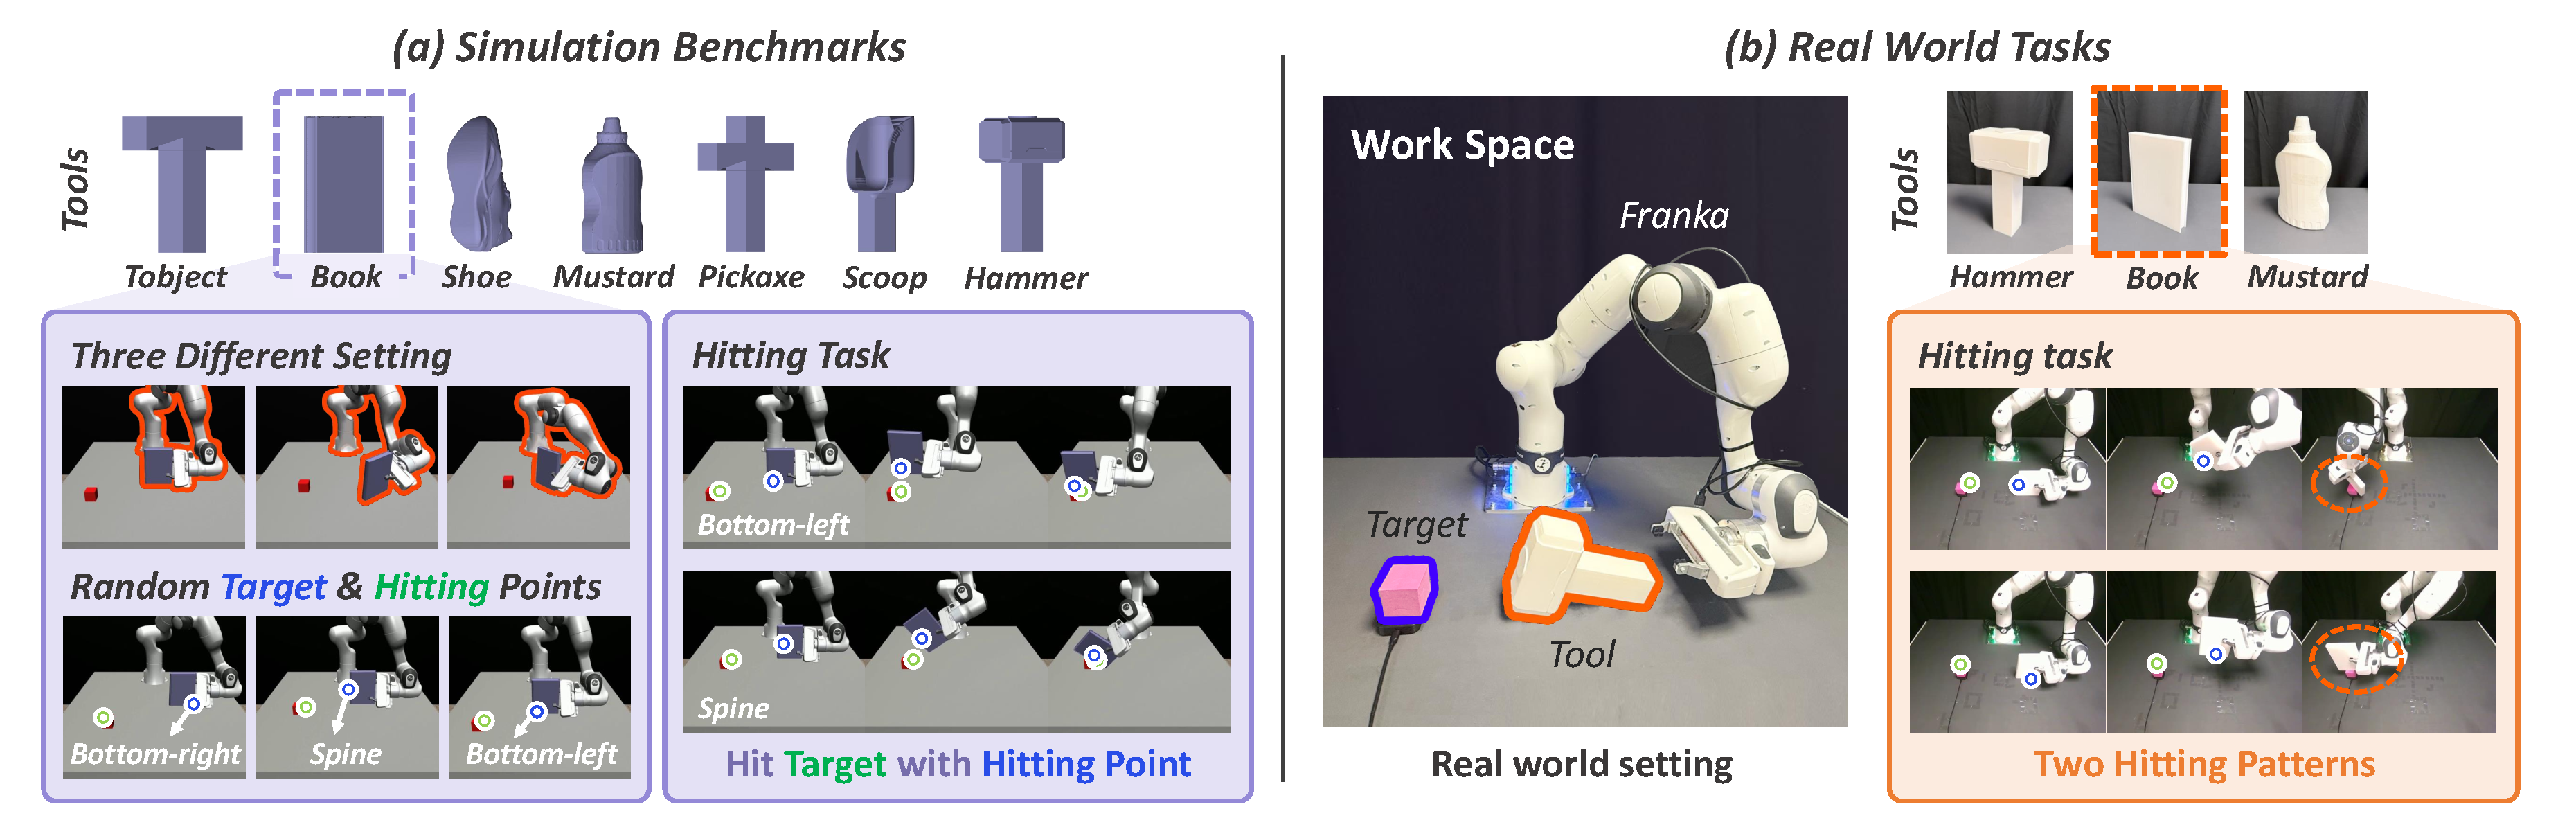
\includegraphics[width=\linewidth]{figures/experiments_settings.pdf}
    \caption{
    \textbf{Simulation Benchmark and Real-world Setting.} (a) The simulation benchmark contains seven tools, three initial settings per tool, and randomized target and hitting points. (b) The real-world setting uses a Franka robot and includes three tools, each with two hitting patterns.
    }
    \label{fig:experiment_settings}
\end{figure}
\section{Experiments}
\label{sec:experiments}

% \lw{We design our experiments to test four hypotheses that together validate the central claims of this work.
% \begin{itemize}[leftmargin=*]
%     \item \textbf{H1: End-to-end policies fail at functional generalization; an intermediate representation is necessary.} Tested by the main comparison against FM and DP (Tab.~\ref{tab:simulation_results}).
%     \item \textbf{H2: Among candidate intermediate representations, 2D keypoint trajectories best balance affordance expressiveness and action groundability.} Tested by the representation ablation (Tab.~\ref{tab:ablation_intermediate_representation}).
%     \item \textbf{H3: Keypoint trajectories must be function-aware; generic keypoint tracking is not enough.} Tested by the comparison against ATM, which uses pretrained generic keypoints (Tab.~\ref{tab:simulation_results}).
%     \item \textbf{H4: The two-stage design generalizes under moderate action-labeled tool diversity, making it a practical recipe for tool-use learning.} Tested by the tool-diversity ablation (Tab.~\ref{tab:ablation_tool_generalization_setting}).
% \end{itemize}}

Functional generalization remains a largely underexplored problem in robotic manipulation.
In this work, we instantiate it with the hitting function and construct both simulation and real-world benchmarks to systematically evaluate whether a policy can transfer the same function to unseen tools. Specifically, we design experiments to test four hypotheses that together validate the central claims of this work:
\begin{itemize}[leftmargin=*]
    \item \textbf{H1}: Functional generalization requires an intermediate representation, not end-to-end mapping.
    %Tested by the main comparison against FM and DP (Tab.~\ref{tab:simulation_results}).
    \item \textbf{H2}: Among candidate intermediate representations, 2D keypoint trajectories best balance affordance expressiveness and action groundability.
    % Tested by the representation ablation (Tab.~\ref{tab:ablation_intermediate_representation}).
    \item \textbf{H3}: Keypoint trajectories must be function-aware; generic keypoint tracking is not enough.
    % Tested by the comparison against ATM, which uses pretrained generic keypoints (Tab.~\ref{tab:simulation_results}).
    \item \textbf{H4}: The two-stage design generalizes under moderate action-labeled tool diversity, making it a practical recipe for tool-use learning.
    % Tested by the tool-diversity ablation (Tab.~\ref{tab:ablation_tool_generalization_setting}).
\end{itemize}

\subsection{Experimental setup}
% Functional generalization remains a largely underexplored problem in robotic manipulation.
% In this work, we instantiate it with the hitting function and construct both simulation and real-world benchmarks to systematically evaluate whether a policy can transfer the same function to unseen tools. \lw{move to first paragraph}



%\paragraph{Simulation Benchmark.}
\textbf{Simulation Benchmark.}~~
% As shown in Fig.~\ref{fig:experiment_settings}, our simulation benchmark contains seven tools, each with three different initial settings.
% For each setting, we collect 30 demonstrations, resulting in 630 samples in total.
% In each sample, the positions of the target cube and the tool-specific hitting point are randomly initialized.
% Our main setting trains all methods on four tools, including hammer, tobject, pickaxe, and mustard, and evaluates their functional generalization performance on the remaining three unseen tools.
% During evaluation, a rollout is considered successful only when the tool strikes the target cube using the designated hitting point.
%For each tool-setting pair, we  \lw{how do we collect data? add MPPI here} 30 demonstrations, resulting in 630 demonstrations in total.
As shown in Fig.~\ref{fig:experiment_settings}, our simulation benchmark contains 7 tools, each with 3 different initial settings. 
For each tool-setting pair, we collect 30 demonstrations using a four-stage Model Predictive Path Integral (MPPI) planner, resulting in 630 demonstrations in total. The MPPI planner generates an action trajectory by optimizing stage-dependent objectives that sequentially encourage the robot to lift the tool, move it toward the target, align the tool-specific hitting point with the target cube, and execute the final strike. In each demonstration, we randomly initialize the target cube position and sample the tool-specific hitting point along the tool boundary, requiring the policy to adapt its motion to both the tool geometry and the target location. In the main setting, all methods are trained on 4 tools, including hammer, tobject, pickaxe, and mustard, and evaluated on the remaining 3 unseen tools. During evaluation, each unseen tool is tested under three initial settings with 30 rollout episodes. A rollout is considered successful only if the robot strikes the target cube using the designated hitting point.



% \paragraph{Real-World Setting.}
\textbf{Real-World Setting.}~~
% Our real-world setting is constructed on a Franka robot platform and includes three tools: hammer, mustard, and book.
% As shown in Fig.~\ref{fig:experiment_settings}, each tool contains two hitting patterns, and each pattern contains 20 expert demonstrations, resulting in 120 real-world trajectories.
% We train the policy on hammer and mustard data and evaluate its functional generalization ability on the unseen book tool.
% A trial is considered successful only if the robot uses the specified hitting pattern to strike the target cube.
% \lw{sys2 data is action free, we can use human videos to collect data}
We further construct a real-world benchmark on a Franka robot platform, as shown in Fig.~\ref{fig:experiment_settings}. 
The real-world setting contains 3 tools: hammer, mustard, and book. 
Each tool has two hitting patterns, and each pattern contains 20 expert demonstrations, resulting in 120 real-world trajectories.
We train the policy on hammer and mustard and evaluate its functional generalization ability on the unseen book tool. 
For each hitting pattern, we perform 20 real-world rollout trials. A trial is successful if the robot follows the specified hitting pattern and strikes the target.

\textbf{Baselines.}~~We compare \algoname{} against three baselines covering end-to-end and keypoint-based policies. \textit{Flow-Matching (FM)}~\cite{lipmanflow} and \textit{Diffusion Policy (DP)}~\cite{chi2025diffusion} are end-to-end visuomotor policies that map observations directly to actions, serving as references for the perception-to-action gap (Sec.~\ref{sec:intro}). \textit{ATM}~\cite{wen2023any} also conditions on keypoint trajectories, but obtains them from a generic tracker pretrained on LIBERO-90 rather than a function-aware predictor, allowing us to test whether the gain comes from using keypoints or from predicting function-aware keypoint motion. All baselines receive the same inputs as \algoname{}: visual observations, proprioceptive states, and the initial hitting and target point positions.

%\paragraph{Evaluation Metrics.}
\textbf{Evaluation Metrics.}~~
All experiments report the success rate (SR) as the main evaluation metric, which is defined as the number of successful trials divided by the total number of rollout trials.

% For a fair comparison, in both simulation and real-world experiments, all policies are given the same input conditions, including visual observations, robot proprioceptive states, and the initial positions of the hitting point and target point.


% \begin{table}[t]
% \centering
% \caption{Performance comparison on simulation and real-world tools.}
% \label{tab:exp_main_results}
% \resizebox{0.8\linewidth}{!}{
% \begin{tabular}{lccccc}
% \toprule
% \multirow{2}{*}{Method} 
% & \multicolumn{4}{c}{Simulation Tools} 
% & \multicolumn{1}{c}{Real-World Tools} \\
% \cmidrule(lr){2-5} \cmidrule(lr){6-6}
% & Scoop & Shoe & Book & Avg. & Book \\
% \midrule
% Flow-Matching    & 0.07 & 0.03 & 0.16 & 0.09 & -- \\
% Diffusion Policy & 0.18 & 0.08 & 0.27 & 0.17 & -- \\
% \hline
% ATM              & -- & -- & -- & -- & -- \\
% \hline
% \algoname{} (Ours)      & 0.42 & 0.23 & 0.42 & 0.36 & -- \\
% \bottomrule
% \end{tabular}
% }
% \end{table}


% \begin{table}[ht]
% \centering
% \caption{\textbf{Simulation Results.} We conduct experiments on three unseen tools, including Scoop, Shoe, and Book. Each unseen tool contains three different initial settings. We perform 30 rollout episodes for each setting and report the success rate.}
% \label{tab:simulation_results}
% \resizebox{0.9\linewidth}{!}{
% \begin{tabular}{lcccccccccc}
% \toprule
% \multirow{2}{*}{Method} 
% & \multicolumn{3}{c}{Scoop} 
% & \multicolumn{3}{c}{Shoe} 
% & \multicolumn{3}{c}{Book} 
% & \multirow{2}{*}{Avg} \\
% \cmidrule(lr){2-4} 
% \cmidrule(lr){5-7} 
% \cmidrule(lr){8-10}
% & S01 & S02 & S03 
% & S01 & S02 & S03 
% & S01 & S02 & S03 
% & \\
% \midrule
% Flow-Matching 
% & 0.00 & 0.03 & 0.17 
% & 0.00 & 0.07 & 0.03 
% & 0.13 & 0.17 & 0.17 
% & \cellcolor{gray!15}0.09 \\

% DP 
% & 0.13 & 0.13 & 0.27 
% & 0.00 & 0.13 & 0.10 
% & 0.33 & \textbf{0.23} & 0.23 
% & \cellcolor{gray!15}0.17 \\

% \midrule
% ATM 
% & 0.13 & 0.17 & 0.07 
% & 0.10 & 0.00 & 0.07 
% & 0.07 & 0.07 & 0.03 
% & \cellcolor{gray!15}0.08 \\

% \midrule
% \algoname{} (Ours) 
% & \textbf{0.30} & \textbf{0.30} & \textbf{0.67} 
% & \textbf{0.23} & \textbf{0.23} & \textbf{0.23} 
% & \textbf{0.53} & 0.20 & \textbf{0.53} 
% & \cellcolor{gray!18}\textbf{0.36} \\
% \bottomrule
% \end{tabular}
% }
% \end{table}

\begin{table}[ht]
\centering
\caption{\textbf{Simulation Results.} Success rate (SR) on three unseen tools. Each setting is evaluated with 30 rollouts, and setting-level SR, tool-level average SR, and overall average SR are reported.}
\label{tab:simulation_results}
\resizebox{\linewidth}{!}{
\begin{tabular}{lccccccccccccc}
\toprule
\multirow{2}{*}{Method} 
& \multicolumn{4}{c}{Scoop} 
& \multicolumn{4}{c}{Shoe} 
& \multicolumn{4}{c}{Book} 
& \multirow{2}{*}{Overall} \\
\cmidrule(lr){2-5} 
\cmidrule(lr){6-9} 
\cmidrule(lr){10-13}
& S01 & S02 & S03 & Avg.
& S01 & S02 & S03 & Avg.
& S01 & S02 & S03 & Avg.
& \\

\midrule
FM~\cite{lipmanflow} 
& 0.00 & 0.03 & 0.17 & \cellcolor{gray!15}0.07
& 0.00 & 0.07 & 0.03 & \cellcolor{gray!15}0.03
& 0.13 & 0.17 & 0.17 & \cellcolor{gray!15}0.16
& \cellcolor{teal!10}0.09 \\

DP~\cite{chi2025diffusion} 
& 0.13 & 0.13 & 0.27 & \cellcolor{gray!15}0.18
& 0.00 & 0.13 & 0.10 & \cellcolor{gray!15}0.08
& 0.33 & \textbf{0.23} & 0.23 & \cellcolor{gray!15}0.26
& \cellcolor{teal!10}0.17 \\

\midrule
ATM~\cite{wen2023any} 
& 0.13 & 0.17 & 0.07 & \cellcolor{gray!15}0.12
& 0.10 & 0.00 & 0.07 & \cellcolor{gray!15}0.06
& 0.07 & 0.07 & 0.03 & \cellcolor{gray!15}0.06
& \cellcolor{teal!10}0.08 \\

\midrule
\algoname{} (Ours) 
& \textbf{0.30} & \textbf{0.30} & \textbf{0.67} & \cellcolor{gray!18}\textbf{0.42}
& \textbf{0.23} & \textbf{0.23} & \textbf{0.23} & \cellcolor{gray!18}\textbf{0.23}
& \textbf{0.53} & 0.20 & \textbf{0.53} & \cellcolor{gray!18}\textbf{0.42}
& \cellcolor{teal!10}\textbf{0.36} \\
\bottomrule
\end{tabular}
}
\end{table}


\begin{figure}[ht]
    \centering
    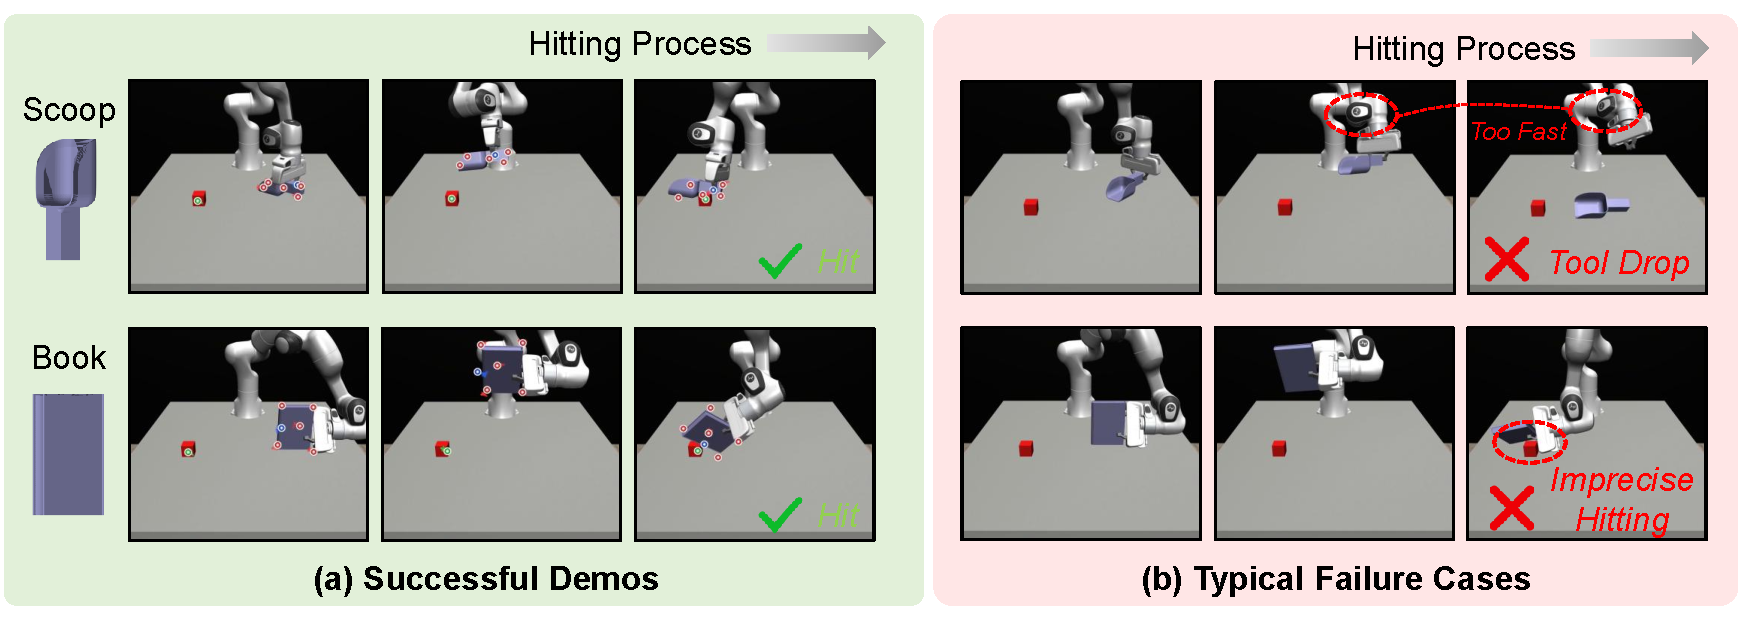
\includegraphics[width=1.0\linewidth]{figures/qualitative-results.pdf}
    \caption{\textbf{Qualitative results of \algoname{}.} (a) Successful demos with predicted keypoint-based functional plans on unseen tools. (b) Two typical failure cases of \algoname{}.}

    \label{fig:qualitative-analysis}
\end{figure}


\begin{figure}[t]
    \centering
    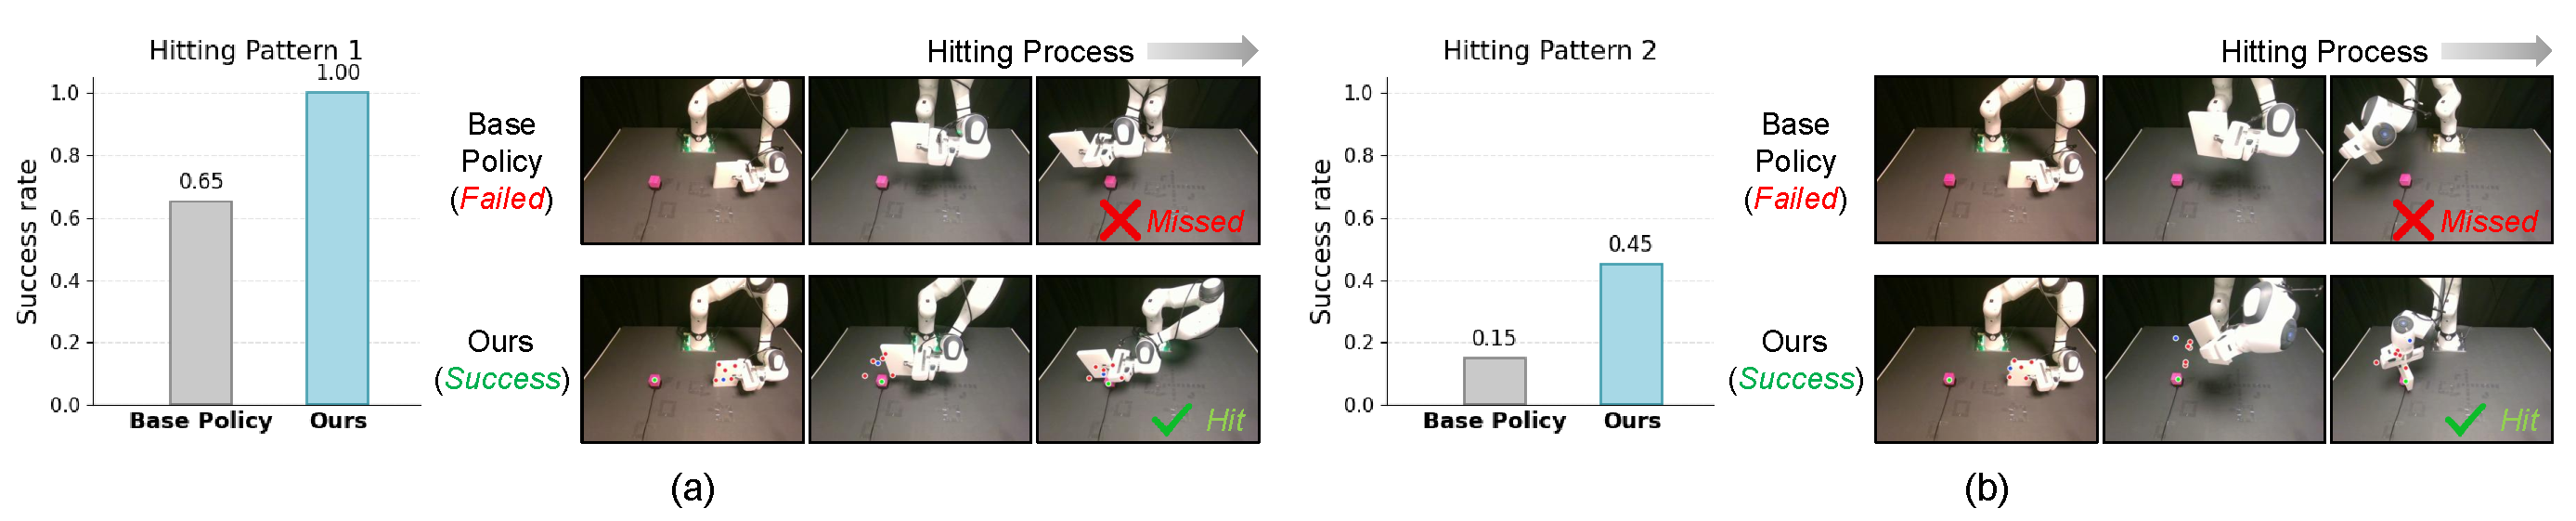
\includegraphics[width=1.0\linewidth]{figures/real-world-exp.pdf}
    \caption{\textbf{Real-World Results.} Results on the unseen book across two hitting patterns. We compare \algoname{} with the FM base policy. Results for hitting with (a) the bottom. (b) the spine.}
    \label{fig:real-world-results}
\end{figure}



% \subsection{Main Results \lw{\& Analysis}}
\subsection{Main Results \& Analysis}

% We compare \algoname{} with state-of-the-art diffusion-based and flow-matching-based policy learning methods. For a fair comparison, all methods are trained with the same input conditions, including visual observations, robot proprioceptive states, and the initial positions of the hitting point and target point. We train all methods on samples from four tools, including hammer, tobject, dtobject, and mustard, and evaluate their generalization performance on the remaining three unseen tools.


%\paragraph{Simulation Results.}
% \textbf{Simulation Results.}~~ We compare \algoname{} with Flow-Matching (FM)~\cite{lipmanflow}, Diffusion Policy (DP)~\cite{chi2025diffusion}, and the keypoint-based policy ATM~\cite{wen2023any}. For a fair comparison, all policies take the same inputs, including observations, robot proprioceptive states, and initial keypoints.
% As shown in Tab.~\ref{tab:simulation_results}, both FM and DP show limited performance on hitting-function generalization, indicating that directly mapping visual observations to actions struggles to transfer across tools.
% For ATM, we use its tracking module pretrained on LIBERO-90 and only fine-tune the track-guided policy on our benchmark.
% Since the pretrained tracking module lacks prior knowledge of the hitting function, it cannot effectively reason about function-relevant keypoint trajectories to guide the low-level policy, even with initial keypoints.
% In contrast, through action-free pretraining, \algoname{} learns the underlying intent of the hitting function and predicts structured functional plans that generalize across tools. By grounding these plans into precise actions, \algoname{} substantially improves the success rate on unseen tools, outperforming the second-best method (DP) by 19\% in overall SR.

% %\paragraph{Real-World Results.} 
% \textbf{Real-World Results.}~~We further compare \algoname{} with the Base Policy (FM) in the real world.
% As shown in Fig.~\ref{fig:real-world-results}, \algoname{} consistently outperforms FM under both hitting patterns.
% The typical failure cases show that, relying only on observations, FM struggles to align the hitting region of novel tools with the target, leading to missed hits.
% In contrast, guided by the predicted keypoint-based functional plans, \algoname{} achieves more accurate alignment and completes the hitting task.

\textbf{Simulation Results.}~~As shown in Tab.~\ref{tab:simulation_results}, FM and DP achieve only $0.09$ and $0.17$ average SR on unseen tools, validating \textbf{H1}: without an intermediate representation exposing the contact region and its alignment with the target, end-to-end policies fall back on the motor patterns of the most visually similar seen tool. 
ATM also underperforms ($0.08$), validating \textbf{H3}: its generic tracker cannot anticipate function-relevant motion, so the keypoint trajectories it provides fail to describe how the contact region should approach the target. 
In contrast, \algoname{} achieves $0.36$, outperforming DP by over $2\times$ with consistent gains across all three unseen tools, and Fig.~\ref{fig:qualitative-analysis}~(a) shows that its predicted keypoint trajectories explicitly bring the tool-specific contact region toward the target before impact. 
We further observe two failure modes (Fig.~\ref{fig:qualitative-analysis}~(b)): \textit{imprecise hitting}, where the 2D trajectories capture the overall motion but lack fine-grained spatial alignment, motivating 3D-aware functional representations; and \textit{tool dropping}, where the execution policy produces jerky actions, motivating smoothness regularization or trajectory post-processing.


% \textbf{Simulation Results.}
% As shown in Tab.~\ref{tab:simulation_results}, the end-to-end policies FM and DP achieve limited success rates on unseen tools. This validates \textbf{H1}, showing that directly mapping visual observations to actions is insufficient for functional generalization. Although the unseen tools share the same hitting function as the seen tools, their geometries, hitting regions, and required motions differ substantially. As a result, FM and DP often fail to infer how the tool-specific hitting region should be aligned with the target, leading to missed hits or incorrect contacts.
% The poor performance of ATM further validates \textbf{H3}, indicating that generic keypoint tracking alone is not enough for functional tool-use generalization. Although ATM guides the policy on keypoint trajectories, its tracker is pretrained on general manipulation data and does not explicitly encode the hitting function. Therefore, the predicted trajectories fail to describe task-relevant functional motion, such as moving the correct contact region toward the target before impact.
% In contrast, our \algoname{} achieves the best performance, outperforming the second-best baseline DP by 19 \%.
% As shown in Fig.~\ref{fig:qualitative-analysis}, \algoname{} succeeds by predicting function-relevant keypoint trajectories that explicitly guide the hitting motion on unseen tools. On the scoop and book, the predicted keypoints describe how the tool-specific hitting points should approach and align with the target before contact. This structured intermediate representation reduces the ambiguity of direct perception-to-action mapping and enables the grounded execution policy $\pi_{\mathrm{sys1}}$ to generate precise actions for successful hitting.
% We further analyze two representative failure cases of our \algoname{}. First, imprecise hitting occurs when the predicted 2D keypoint trajectories capture the overall hitting motion but are not accurate enough for fine-grained spatial alignment. Second, tool dropping occurs when the execution policy grounds the trajectories into unstable or jerky actions. These failures suggest two future directions: more spatially accurate, 3D-aware functional representations for functional reasoning, and smoother action grounding through training-time smoothness regularization or post-processing-based trajectory refinement.
%Through action-free pretraining, keypoints motion predictor $\pi_{\mathrm{sys2}}$ predicts structured keypoint trajectories that describe how the tool-specific hitting point should move and align with the target. The grounded execution policy $\pi_{\mathrm{sys1}}$ then grounds these predicted trajectories into executable robot actions. As shown in Fig.~\ref{fig:qualitative-analysis}, on unseen tools, such as the scoop and book, \algoname{} predicts meaningful keypoint motions and successfully completes the hitting task, demonstrating that the intermediate plan effectively bridges functional reasoning and action execution.

\textbf{Real-World Results.}~~
% We further compare \algoname{} with the FM base policy in the real world, using the unseen book tool under two hitting patterns.
% As shown in Fig.~\ref{fig:real-world-results}, \algoname{} achieves higher success rates than FM in both settings.
% Together with the visualized failure cases, these results further validate \textbf{H1}: directly mapping observations to actions struggles to transfer the same function to a novel tool whose geometry, contact region, and required motion differ from the training tools.
% Specifically, FM often misses the target because it fails to align the appropriate hitting region of the book before contact.
% By contrast, \algoname{} predicts keypoint-based functional plans that describe how the book should move toward and strike the target, allowing the execution policy to generate more accurate actions for successful hitting.
We further evaluate whether \algoname{} can transfer the learned hitting function to the real world by comparing it with the FM base policy on the unseen book tool.
As shown in Fig.~\ref{fig:real-world-results}, \algoname{} consistently outperforms FM under both hitting patterns.
This further supports \textbf{H1}, showing that direct perception-to-action mapping is insufficient for functional generalization. As illustrated by the failure cases in Fig.~\ref{fig:real-world-results}, FM often fails to align the correct hitting region of the unseen book tool with the target, leading to missed hits.
In contrast, \algoname{} predicts function-relevant keypoint trajectories that specify how the desired hitting region should approach and contact the target.
These intermediate plans provide explicit guidance for the grounded execution policy, enabling more accurate alignment and successful real-world hitting.
















% These results further demonstrate the effectiveness of our decoupled functional planning and action execution design in real-world tool-use scenarios.

% \begin{table}[t]
% \centering
% \caption{Ablation study on different trade-off representations.}
% \label{tab:ablation_intermediate_representation}
% \resizebox{0.6\linewidth}{!}{
% \begin{tabular}{lcccc}
% \toprule
% Representation & Scoop & Shoe & Book & Avg. \\
% \midrule
% Flow-Matching         & 0.07 & 0.03 & 0.16 & \cellcolor{gray!18} 0.09 \\
% \midrule
% + Affordance Images     & 0.34 & 0.11 & 0.16 & \cellcolor{gray!18} 0.20 \\
% + Human Video Prompts   & 0.26 & 0.09 & 0.23 & \cellcolor{gray!18} 0.19 \\
% + Keypoint Trajectories & 0.50 & 0.31 & 0.67 & \cellcolor{gray!18} 0.49 \\
% \bottomrule
% \end{tabular}
% }
% \end{table}

% \begin{table}[t]
% \centering
% \caption{Ablation study on different trade-off representations.}
% \label{tab:ablation_intermediate_representation}
% \resizebox{0.6\linewidth}{!}{
% \begin{tabular}{lcccc}
% \toprule
% Representation & Scoop & Shoe & Book & Avg. \\
% \midrule
% Flow-Matching         & 0.07 & 0.03 & 0.16 & \cellcolor{gray!18} 0.09 \\
% \midrule
% + Aff. Images     & 0.34 & 0.11 & 0.16 & \cellcolor{gray!18} 0.20 \\
% + Hum. Vid. Prompts   & 0.26 & 0.09 & 0.23 & \cellcolor{gray!18} 0.19 \\
% + Key. Trajectories & 0.50 & 0.31 & 0.67 & \cellcolor{gray!18} 0.49 \\
% \bottomrule
% \end{tabular}
% }
% \end{table}


% \begin{table}[t]
% \centering
% \caption{Ablation study on the number of keypoints.}
% \label{tab:ablation_num_keypoints}
% \resizebox{0.5\linewidth}{!}{
% \begin{tabular}{lcccc}
% \toprule
% \# Keypoints & Scoop & Book & Shoe & Avg. \\
% \midrule
% 5 & -- & -- & -- & -- \\
% 7 & -- & -- & -- & -- \\
% 9 & -- & -- & -- & -- \\
% \bottomrule
% \end{tabular}
% }
% \end{table}

\subsection{Ablation Studies}

% \lw{
% \textbf{Ablation Settings.}~~Beyond comparing against baselines, we conduct two ablations to dissect the design choices behind \algoname{}. The first ablation varies the functional intermediate representation, conditioning the same execution policy on affordance images, human video prompts, or 2D keypoint trajectories, to identify which representation best balances affordance expressiveness and action groundability. The second ablation varies the diversity of action-labeled tools, training \algoname{} on 1, 4, or 6 tools and testing on the remaining unseen ones, to study how much action-labeled data is needed to ground the function-aware plans learned from action-free pretraining.}


% \textbf{Ablation Settings.}~~
Beyond comparing against baselines, we conduct two ablations to dissect the design choices behind \algoname{}. The first ablation varies the functional intermediate representation, conditioning the execution policy on affordance images, human video prompts, or 2D keypoint trajectories, to identify which representation best balances affordance expressiveness and action groundability. The second ablation varies the diversity of action-labeled tools, training \algoname{} on 1, 4, or 6 tools and testing on the unseen tools, to evaluate whether the two-stage pipeline provides a practical recipe for functional generalization using moderate robotic data.



% Our ablation studies try to answer three questions: 
% (1) Which type of functional intermediate representation provides the strongest functional generalization capability? 
% (2) How does the number of keypoints affect the performance of \algoname{}? 
% (3) How well does \algoname{} perform across different levels of functional generalization?

% Our ablation studies try to answer the following questions:
% \begin{itemize}[leftmargin=*]
%     \item Which functional intermediate representation best supports functional generalization?
%     % \item How does the number of keypoints affect the performance of \algoname{}?
%     \item How does \algoname{} perform under different levels of functional generalization?
% \end{itemize}


% Our ablation studies try to answer two questions. \textbf{Q1:} Which functional intermediate representation best supports functional generalization? \textbf{Q2:} How does the diversity of action-labeled training tools affect functional grounding and generalization? \lw{merge to previous hypothesis}

% \textbf{Q2:} How does \algoname{} perform under different levels of functional generalization?



\subsubsection{Effect of Functional Intermediate Representations.}

\begin{wraptable}{r}{0.55\linewidth}
\vspace{-1.0em}
\centering
\caption{\textbf{Ablation Results on Functional Intermediate Representations.} We condition FM on different representations and report the SR on 3 unseen tools.}
\label{tab:ablation_intermediate_representation}
\resizebox{0.95\linewidth}{!}{
\begin{tabular}{lcccc}
\toprule
Representation & Scoop & Shoe & Book & Avg. \\
\midrule
Flow-Matching & 0.07 & 0.03 & 0.16 & \cellcolor{teal!10} 0.09 \\
\midrule
+ Aff. Images & 0.34 & 0.11 & 0.16 & \cellcolor{teal!10} 0.20 \\
+ Hum. Vid. Prompts & 0.26 & 0.09 & 0.23 & \cellcolor{teal!10} 0.19 \\
+ Key. Trajectories & 0.50 & 0.31 & 0.67 & \cellcolor{teal!10} 0.49 \\
\bottomrule
\end{tabular}
}
\vspace{-1.0em}
\end{wraptable}

As discussed in Sec.~\ref{sec:Functional Intermediate Representations Selection}, we investigate the effect of different functional intermediate representations by directly training the execution policy $\pi_{\mathrm{sys1}}$. 
% The results are summarized in Tab.~\ref{tab:ablation_intermediate_representation}. 
Results in Tab.~\ref{tab:ablation_intermediate_representation} show that introducing affordance images or human video prompts improves generalization, suggesting that tool-region cues and visual motion demonstrations of the hitting provide useful functional information.
In comparison, 2D keypoint trajectories capture fine-grained hitting and target point information while explicitly describing structured functional motion over time. These results support \textbf{H2}: keypoint trajectories provide a more compact and action-groundable condition, leading to the best functional generalization.


\begin{table}[ht]
\centering
\caption{\textbf{Ablation on Action-Labeled Tool Diversity.} Success rate (SR) of \algoname{} under different training-to-testing tool splits. `M-to-N' denotes training on $M$ tools and testing on $N$ unseen tools.}


\label{tab:ablation_tool_generalization_setting}
\resizebox{0.9\linewidth}{!}{
\begin{tabular}{lcccccccc}
\toprule
\multirow{2}{*}{Method}
& \multicolumn{8}{c}{Tools} \\
\cmidrule(lr){2-9}
& Hammer & Tobject & Pickaxe & Mustard & Scoop & Shoe & Book & Avg. \\
\midrule
\algoname{} (1-to-6) & -- & 0.26 & 0.34 & 0.17 & 0.14 & 0.10 & 0.23 & \cellcolor{teal!10} 0.21 \\
\algoname{} (4-to-3) & -- & -- & -- & -- & 0.42 & 0.23 & 0.42 & \cellcolor{teal!10} 0.36 \\
\algoname{} (6-to-1) & -- & -- & -- & -- & -- & -- & 0.52 & \cellcolor{teal!10} 0.52\\
\bottomrule
\end{tabular}
}
\end{table}

% \subsubsection{Effect of Action-Labeled Tool Diversity.} \lw{what is this experiment trying to show?}
% Beyond the standard 4-to-3 generalization setting, we further evaluate two settings, where \algoname{} is fine-tuned with robotic data from 1 or 6 tools and tested on the 6 or 1 unseen tools, respectively.
% As shown in Tab.~\ref{tab:ablation_tool_generalization_setting}, using robotic data from only one tool leads to a performance drop on novel tools, indicating that limited action-labeled diversity is insufficient for grounding structured functional plans into motor commands.
% In contrast, increasing the diversity of action-labeled training tools improves action grounding and leads to higher unseen-tool success rates, with the 6-to-1 setting achieving the best performance.
% These results reveal a practical trade-off: too little robotic data limits action grounding, while collecting demonstrations for many tools increases the data-collection burden.
% Consequently, the non-trivial performance under the balanced 4-to-3 setting suggests a practical generalization paradigm: scalable action-free data enhances the policy's cross-tool generalization ability, while moderate action-labeled data is sufficient for learning action grounding.

%\subsubsection{Effect of Action-Labeled Tool Diversity.}
%Beyond the standard 4-to-3 generalization setting, we further evaluate two settings, where \algoname{} is fine-tuned with robotic data from 1 or 6 tools and tested on the remaining 6 or 1 unseen tools, respectively.
%As shown in Tab.~\ref{tab:ablation_tool_generalization_setting}, using robotic data from only one tool leads to a performance drop on novel tools, indicating that limited action-labeled diversity is insufficient for reliably grounding structured functional plans into motor commands.
%In contrast, increasing the diversity of action-labeled training tools improves action grounding and leads to higher unseen-tool success rates, with the 6-to-1 setting achieving the best performance.
%These results reveal a practical trade-off: too little robotic data limits action grounding, while collecting demonstrations for many tools increases the data-collection burden.
%Consequently, the non-trivial performance under the balanced 4-to-3 setting supports \textbf{H4}, suggesting that the two-stage design of \algoname{} provides a practical recipe for tool-use learning: scalable action-free data supports cross-tool functional reasoning, while moderate action-labeled data enables effective grounding of the predicted trajectories into executable actions.

\subsubsection{Effect of Action-Labeled Tool Diversity.}
Beyond the standard 4-to-3 setting, we evaluate \algoname{} fine-tuned with robotic data from 1 or 6 tools and tested on the unseen ones. As shown in Tab.~\ref{tab:ablation_tool_generalization_setting}, the success rate grows monotonically with action-labeled tool diversity, from $0.21$ (1-to-6) to $0.36$ (4-to-3) to $0.52$ (6-to-1), confirming that broader data coverage improves action grounding. This reveals a practical trade-off: too little robotic data limits grounding, while collecting demonstrations for many tools is costly. The non-trivial 4-to-3 performance supports \textbf{H4}: the two-stage design of \algoname{} provides a practical recipe, where scalable action-free data supports cross-tool functional reasoning and moderate action-labeled data suffices to ground predicted trajectories into executable actions.




% \begin{figure}[ht]
%     \centering
%     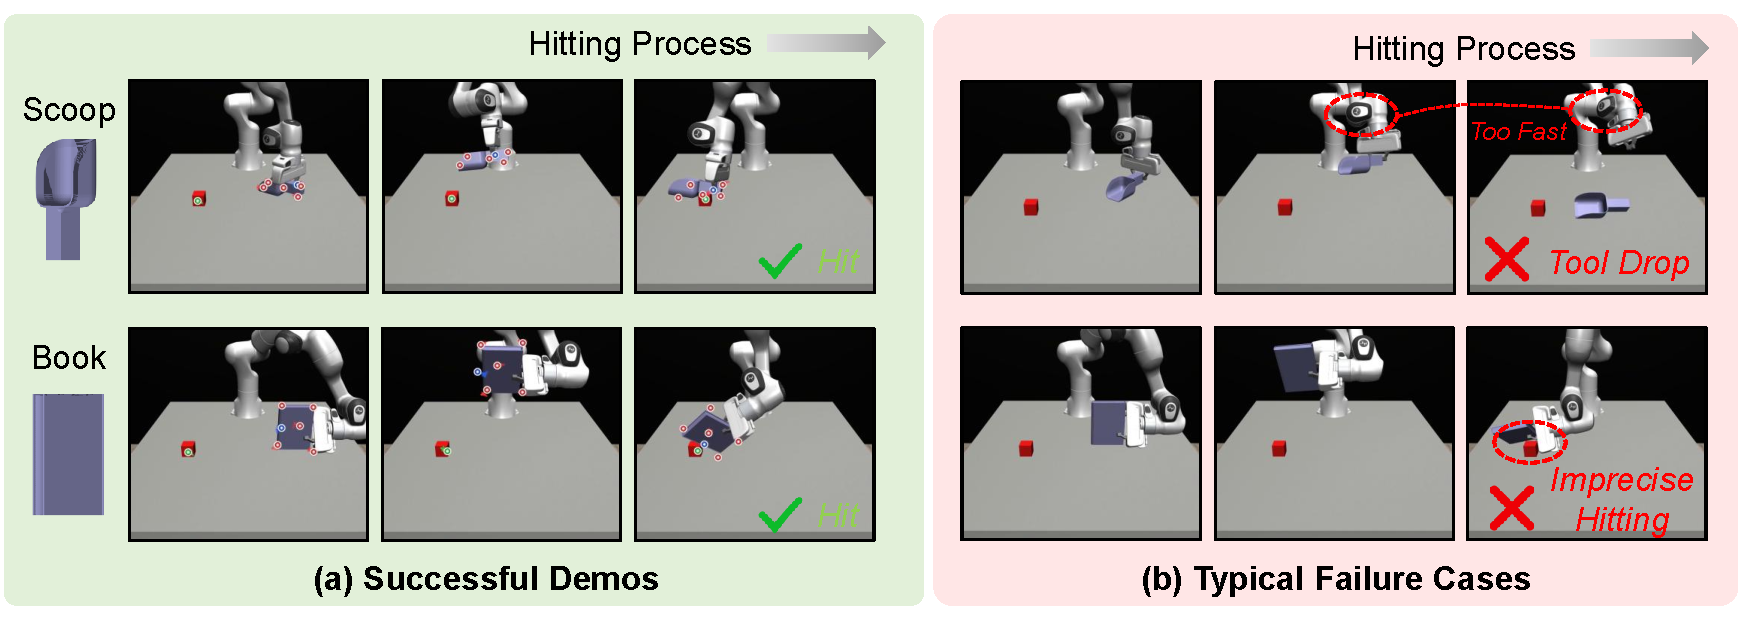
\includegraphics[width=0.95\linewidth]{figures/qualitative-results.pdf}
%     \caption{\textbf{Qualitative results of \algoname{}.} (a) Successful demos with predicted keypoint-based functional plans on unseen tools. (b) Two typical failure cases of \algoname{}.}

%     \label{fig:qualitative-analysis}
% \end{figure}

% \subsection{Qualitative Analysis}

% In this section, we conduct a comprehensive qualitative analysis on the behavior of \algoname{} on unseen tools. 
% As shown in Fig.~\ref{fig:qualitative-analysis}, we first visualize the predicted 2D keypoint-based functional plans of \algoname{} on different unseen tools. 
% We then summarize two representative failure cases from \algoname{}, which provide useful insights for further improvement.

% \subsubsection{Visualization of Functional Plans of \algoname{}.}

% Fig.~\ref{fig:qualitative-analysis}(a) visualizes the functional plans predicted by \algoname{} on unseen tools. 
% Although these tools are not observed during training, \algoname{} can still predict structured keypoint trajectories that reflect the underlying functional intent, such as aligning the hitting point with the target point before contact. 
% Conditioned on these predicted functional plans, the execution policy can ground them into robot actions and successfully complete the hitting task with the designated hitting point. 
% These results show that the learned keypoint-based plans capture transferable functional motion patterns beyond tool-specific appearances.

% \subsubsection{Typical Failure Cases.}

% As shown in Fig.~\ref{fig:qualitative-analysis}(b), we further identify two representative failure modes of our \algoname{}.

% \paragraph{Imprecise hitting.}
% The first failure mode is imprecise hitting. 
% Although \algoname{} can predict a roughly correct hitting trajectory, it may fail to strike the target precisely with the designated hitting point. 
% We conjecture that this limitation comes from the 2D keypoint representation, and exploring 3D-aware functional intermediate representations may further improve the performance.

% \paragraph{Tool dropping.}
% The second failure mode is tool dropping. 
% The low-level execution policy may ground the predicted functional plan into jerky actions, causing the tool to drop from the gripper and eventually fail the hitting task. 
% Introducing additional smoothness constraints during the finetuning of the low-level execution policy or applying post-processing to the predicted actions may help mitigate this problem.

% \subsection{Qualitative Analysis \lw{Failure Analysis}} 

% % We conduct a comprehensive qualitative analysis of \algoname{} on unseen tools and summarize representative failure cases in Fig.~\ref{fig}.

% %\paragraph{Functional Plan Visualization.}
% \textbf{Functional Plan Visualization.}~~
% As shown in Fig.~\ref{fig:qualitative-analysis}~(a), \algoname{} predicts structured keypoint-based functional plans for unseen tools such as the book and scoop. These plans capture transferable functional motion patterns, such as aligning the hitting region with the target before contact. Conditioned on the predicted plans, the execution policy grounds them into robot actions and successfully completes the hitting task with the designated hitting point.

% %\paragraph{Typical Failure Cases.}
% \textbf{Typical Failure Cases.}~~
% Fig.~\ref{fig:qualitative-analysis}~(b) reveals two representative failure modes of \algoname{}. The first is \textit{imprecise hitting}, where \algoname{} predicts a roughly correct hitting trajectory but fails to strike the target precisely with the designated hitting point. This suggests that 2D keypoints may be insufficient for fine-grained spatial alignment, and 3D-aware functional representations may further improve performance. The second is \textit{tool dropping}, where the execution policy grounds the predicted plan into jerky actions and causes the tool to slip from the gripper. This indicates that smoother action grounding or action post-processing may help improve low-level execution robustness.

%===============================================================================
% \section{Conclusion and Limitation}
% \label{sec:conclusion}
\section{Conclusion and Limitation}
\label{sec:conclusion}
In this paper, we identify \textit{functional generalization} as an important yet underexplored problem, where an agent needs to accomplish the same function with unseen tools. 
To address this problem, we propose \algoname{}, a policy that decouples functional reasoning from action execution via an intermediate representation. 
In this way, \algoname{} learns functional intent from action-free data to predict keypoint-based plans, and then grounds them into executable robot actions by fine-tuning on limited action-labeled demonstrations.
We introduce a seven-tool hitting-function benchmark to evaluate functional generalization in simulation and real-world settings. 
Extensive experiments show that \algoname{} improves generalization to unseen tools over state-of-the-art methods. 

\paragraph{Limitations and Future Work.}
% Although this work introduces a new functional generalization problem, our current solution still has several limitations. 
First, the functional-relevant hitting and target points are specified in this study, while future work may leverage vision foundation models~\cite{yuan2025robopoint} or pretrain a keypoint proposal model to automatically identify function-relevant keypoints. 
Second, our pipeline does not consider the grasping process. 
We will extend \algoname{} to predict grasp styles from keypoint-based functional trajectories and study more dedicated end-effectors such as dexterous hands.


% \section{Citations}
% \label{sec:citations}

% 	Citations can be made using either \textbackslash citep\{\} or \textbackslash citet\{\}, depending from the appropriateness. To avoid the citation moving to the next line, it is often a good practice to replace the space before with a tilde (\~{}) character.
% 	Example 1: ``CoRL is the best conference ever~\citep{Gauss1857}.''
% 	Example 2: ``\citet{Lagrange1788} proved, both theoretically and numerically, that CoRL is the best conference ever.''
	
%===============================================================================

% \section{Experimental Results}
% \label{sec:result}

% 	Nam dui ligula, fringilla a, euismod sodales, sollicitudin vel, wisi. Morbi auctor lorem non justo.
% 	Nam lacus libero, pretium at, lobortis vitae, ultricies et, tellus. Donec aliquet, tortor sed accumsan
% 	bibendum, erat ligula aliquet magna, vitae ornare odio metus a mi. Morbi ac orci et nisl hendrerit
% 	mollis. 

% 	Suspendisse ut massa. Cras nec ante. Pellentesque a nulla. Cum sociis natoque penatibus
% 	et magnis dis parturient montes, nascetur ridiculus mus. Aliquam tincidunt urna. Nulla ullamcorper
% 	vestibulum turpis. Pellentesque cursus luctus mauris.
	
% 	Nulla malesuada porttitor diam. Donec felis erat, congue non, volutpat at, tincidunt tristique, libero.
% 	Vivamus viverra fermentum felis. Donec nonummy pellentesque ante. Phasellus adipiscing semper 	elit. 
% 	Proin fermentum massa ac quam. Sed diam turpis, molestie vitae, placerat a, molestie nec, leo.
% 	Maecenas lacinia. Nam ipsum ligula, eleifend at, accumsan nec, suscipit a, ipsum. Morbi blandit
% 	ligula feugiat magna. Nunc eleifend consequat lorem. Sed lacinia nulla vitae enim. Pellentesque tin-
% 	cidunt purus vel magna. Integer non enim. Praesent euismod nunc eu purus. Donec bibendum quam
% 	in tellus. Nullam cursus pulvinar lectus. Donec et mi. Nam vulputate metus eu enim. Vestibulum
% 	pellentesque felis eu massa.
% 	Quisque ullamcorper placerat ipsum. Cras nibh. Morbi vel justo vitae lacus tincidunt ultrices. 
	
% 	Lorem
% 	ipsum dolor sit amet, consectetuer adipiscing elit. In hac habitasse platea dictumst. Integer tempus
% 	convallis augue. Etiam facilisis. Nunc elementum fermentum wisi. Aenean placerat. Ut imperdiet,
% 	enim sed gravida sollicitudin, felis odio placerat quam, ac pulvinar elit purus eget enim. Nunc vitae
% 	tortor. Proin tempus nibh sit amet nisl. Vivamus quis tortor vitae risus porta vehicula.

% %===============================================================================

% \section{Conclusion}
% \label{sec:conclusion}

% 	Nam dui ligula, fringilla a, euismod sodales, sollicitudin vel, wisi. Morbi auctor lorem non justo.
% 	Nam lacus libero, pretium at, lobortis vitae, ultricies et, tellus. Donec aliquet, tortor sed accumsan
% 	bibendum, erat ligula aliquet magna, vitae ornare odio metus a mi. Morbi ac orci et nisl hendrerit
% 	mollis. Suspendisse ut massa. Cras nec ante. Pellentesque a nulla. Cum sociis natoque penatibus
% 	et magnis dis parturient montes, nascetur ridiculus mus. Aliquam tincidunt urna. Nulla ullamcorper
% 	vestibulum turpis. Pellentesque cursus luctus mauris.
% 	Nulla malesuada porttitor diam. Donec felis erat, congue non, volutpat at, tincidunt tristique, libero.
% 	Vivamus viverra fermentum felis. Donec nonummy pellentesque ante. Phasellus adipiscing semper
% 	elit. Proin fermentum massa ac quam. Sed diam turpis, molestie vitae, placerat a, molestie nec, leo.
% 	Maecenas lacinia. Nam ipsum ligula, eleifend at, accumsan nec, suscipit a, ipsum. Morbi blandit
% 	ligula feugiat magna. Nunc eleifend consequat lorem. Sed lacinia nulla vitae enim. Pellentesque tin-
% 	cidunt purus vel magna. Integer non enim. Praesent euismod nunc eu purus. Donec bibendum quam
% 	in tellus. Nullam cursus pulvinar lectus. Donec et mi. Nam vulputate metus eu enim. Vestibulum
% 	pellentesque felis eu massa.
% 	Quisque ullamcorper placerat ipsum. Cras nibh. Morbi vel justo vitae lacus tincidunt ultrices. Lorem
% 	ipsum dolor sit amet, consectetuer adipiscing elit. In hac habitasse platea dictumst. Integer tempus
% 	convallis augue. Etiam facilisis. Nunc elementum fermentum wisi. Aenean placerat. Ut imperdiet,
% 	enim sed gravida sollicitudin, felis odio placerat quam, ac pulvinar elit purus eget enim. Nunc vitae
% 	tortor. Proin tempus nibh sit amet nisl. Vivamus quis tortor vitae risus porta vehicula.

%===============================================================================




\clearpage
\newpage
\bibliographystyle{assets/plainnat}
\bibliography{paper}

\clearpage
\appendix

\phantomsection
\section*{Appendix}


\begin{itemize}
  \item[] \textbf{\ref{app:hitting_benchmarks} Hitting Benchmark Construction and Implementation Details}
    \begin{itemize}
      \item[] \ref{app:fir_extraction} Extraction of Functional Intermediate Representations
      \item[] \ref{app:mppi_annotation} MPPI-based Demonstration Generation
      \item[] \ref{app:implementation_details} Training and Implementation Details
    \end{itemize}
    
  \item[] \textbf{\ref{app:additional_experimental_results} Additional Experimental Results}
    \begin{itemize}
      \item[] \ref{app:more_real_world_experiments} More Real-World Experiments
      \item[] \ref{app:more_qualitative_results} Additional Qualitative Comparisons
    \end{itemize}
\end{itemize}



\section{Hitting Benchmark Construction and Implementation Details}
\label{app:hitting_benchmarks}
This section provides additional details on the construction of our hitting benchmarks. We first describe the extraction of different functional intermediate representations in Appx.~\ref{app:fir_extraction}, then introduce MPPI-based action-label generation in Appx.~\ref{app:mppi_annotation}. Finally, we summarize the training and implementation details of FORGE and all baselines in Appx.~\ref{app:implementation_details}.

\begin{table}[ht]
\centering
\caption{\textbf{Statistics of Functional Intermediate Representations.}
We report the number of tools, settings, initial poses, samples per pose, and total samples for each representation.}
\label{tab:representation_statistics}
\resizebox{\linewidth}{!}{
\begin{tabular}{lccccc}
\toprule
Representation & \# Tools & \# Settings & \# Initial Poses & \# Samples / Pose & \# Total \\
\midrule
Affordance Image & 7 & 1 & 1 & 1 & 7 \\
Human Video Prompts & 7 & 3 & 5 & 5 & 525 \\
Keypoint Trajectories (Simulation) & 7 & 3 & 30 & 1 & 630 \\
Keypoint Trajectories (Real World) & 6 & 2 & 1 & 20 & 240 \\
\bottomrule
\end{tabular}
}
\end{table}

\label{app:fir_extraction}

\begin{figure}[!h]
    \centering
    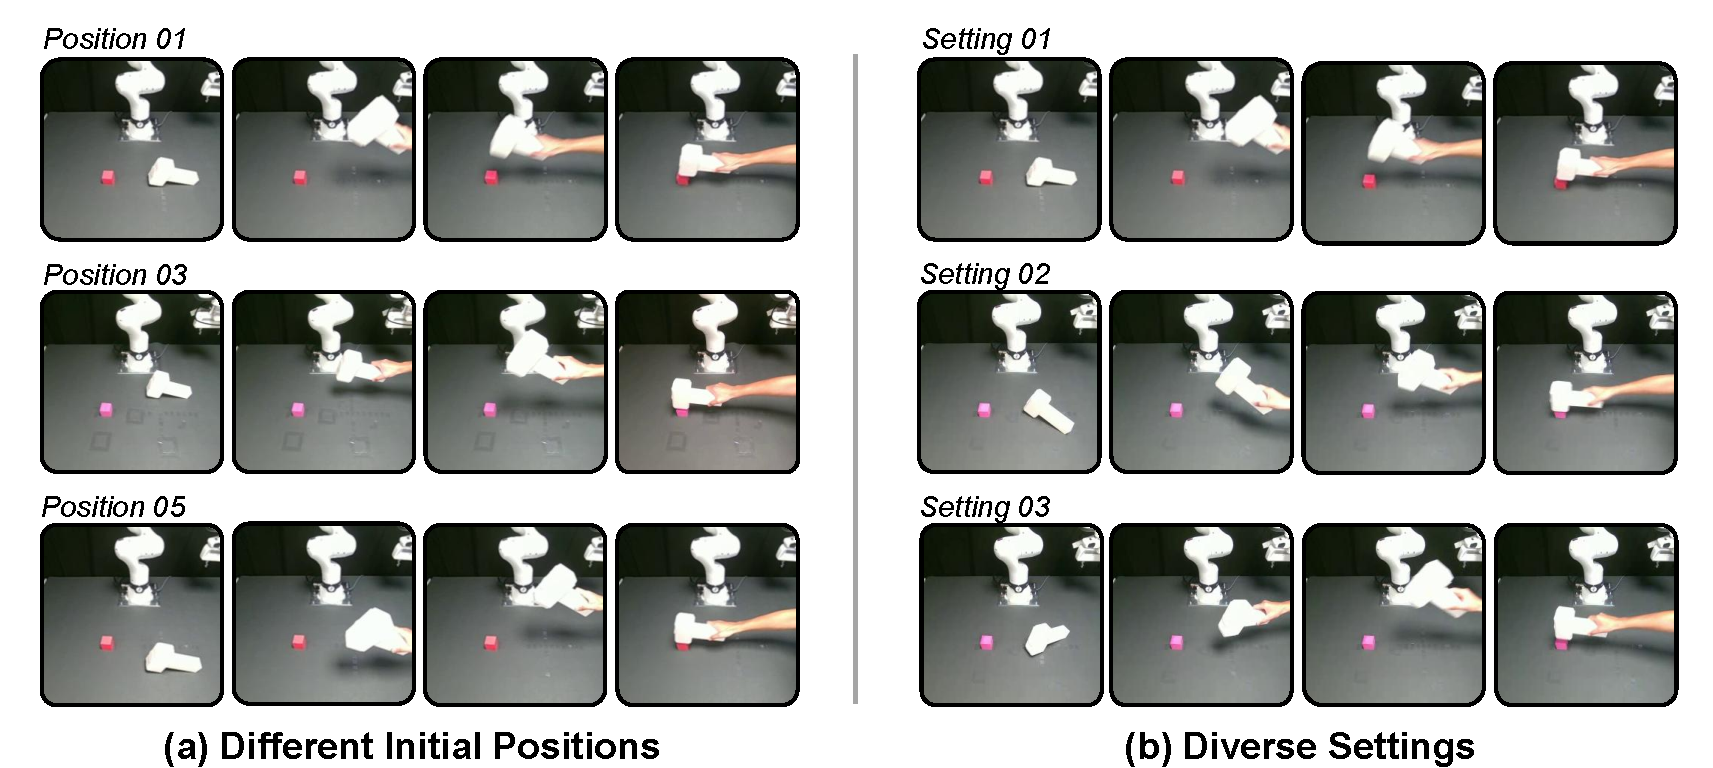
\includegraphics[width=1.0\linewidth]{figures/human-video-prompt.pdf}
    \caption{\textbf{Human Video Prompt Samples.}
    (a) Samples from different initial positions. (b) Samples from different settings.}

    \label{fig:human-video-prompts}
\end{figure}

\subsection{Extraction of Functional Intermediate Representations}
As discussed in Sec.~\ref{sec:Functional Intermediate Representations Selection}, we consider three types of functional intermediate representations: affordance images, human video prompts, and 2D keypoint trajectories. Specifically, we describe how each representation is extracted and incorporated as an additional condition for the grounded execution policy $\pi_{\mathrm{sys1}}$. The statistics of these representations are summarized in Tab.~\ref{tab:representation_statistics}.

\begin{table}[!h]
\centering
\caption{\textbf{Main Reward Terms for MPPI-based Demonstration Generation.}
Here, $d_x$, $d_y$, and $d_{xy}$ denote the distances between the hitting point and the target along the $x$ axis, the $y$ axis, and the $xy$ plane, respectively, while $\Delta d_x$, $\Delta d_y$, and $\Delta d_{xy}$ denote their step-wise reductions.
For the vertical direction, $z_{\mathrm{lift}}$ denotes the tool lifting height from its initial height, $z_1$ denotes the target lifting threshold in Stage~1, $\Delta z_{\mathrm{lift}}$ denotes the step-wise lifting progress, and $e_z$ denotes the error between the current tool height and the target hovering height.
$\Delta z_{\mathrm{head}}$ denotes the vertical displacement of the hitting point between consecutive steps, so $-\Delta z_{\mathrm{head}}$ measures downward motion.
The terms $r_\ast$ reward the current state for satisfying the stage-specific objective, while $r_{\ast\_\mathrm{prog}}$ rewards step-wise progress toward that objective.}

\label{tab:mppi_rewards}
\resizebox{\linewidth}{!}{
\begin{tabular}{lp{0.30\linewidth}p{0.50\linewidth}}
\toprule
Stage & Objective & Main Reward Terms \\
\midrule
Stage 1 
& Lift the tool and align it with the target along the $x$ and $y$ axes.
& 
$
\begin{aligned}
r_{\mathrm{lift}} &= 18.0\min(z_{\mathrm{lift}}, z_1), \\
r_{\mathrm{lift\_prog}} &= 100.0\min(\Delta z_{\mathrm{lift}}, 0.02), \\
r_x &= 22.0\exp(-18.0 d_x), \\
r_{x\_\mathrm{prog}} &= 120.0\min(\Delta d_x, 0.02), \\
r_y &= 8.0\exp(-8.0 d_y), \\
r_{y\_\mathrm{prog}} &= 35.0\min(\Delta d_y, 0.02).
\end{aligned}
$
\\
\midrule
Stage 2 
& Move the tool toward the target while maintaining a suitable hovering height. 
& 
$
\begin{aligned}
r_{xy} &= 14.0\exp(-10.0 d_{xy}), \\
r_x &= 12.0\exp(-18.0 d_x), \\
r_y &= 8.0\exp(-10.0 d_y), \\
r_z &= 7.0\exp(-18.0 e_z), \\
r_{xy\_\mathrm{prog}} &= 95.0\min(\Delta d_{xy}, 0.02), \\
r_{x\_\mathrm{prog}} &= 80.0\min(\Delta d_x, 0.02), \\
r_{y\_\mathrm{prog}} &= 40.0\min(\Delta d_y, 0.02).
\end{aligned}
$
\\
\midrule
Stage 3 
& Finely align the tool-specific hitting point above the target. 
& 
$
\begin{aligned}
r_{xy} &= 14.0\exp(-14.0 d_{xy}), \\
r_x &= 14.0\exp(-24.0 d_x), \\
r_y &= 10.0\exp(-18.0 d_y), \\
r_{xy\_\mathrm{prog}} &= 145.0\min(\Delta d_{xy}, 0.018), \\
r_{x\_\mathrm{prog}} &= 135.0\min(\Delta d_x, 0.018), \\
r_{y\_\mathrm{prog}} &= 110.0\min(\Delta d_y, 0.018), \\
r_z &= 7.0\exp(-18.0 e_z).
\end{aligned}
$
\\
\midrule
Stage 4 
& Keep the hitting point close to the target and execute the downward strike. 
& 
$
\begin{aligned}
r_{xy} &= 12.0\exp(-16.0 d_{xy}), \\
r_x &= 14.0\exp(-28.0 d_x), \\
r_y &= 10.0\exp(-18.0 d_y), \\
r_{xy\_\mathrm{prog}} &= 120.0\min(\Delta d_{xy}, 0.015), \\
r_{x\_\mathrm{prog}} &= 100.0\min(\Delta d_x, 0.015), \\
r_{y\_\mathrm{prog}} &= 80.0\min(\Delta d_y, 0.015), \\
r_{\mathrm{hit}} &= 150.0\min(-\Delta z_{\mathrm{head}}, 0.05),
\end{aligned}
$
\\
\midrule
Contact / Success 
& Encourage valid downward contact with the target.
& 
$
\begin{aligned}
r_{\mathrm{contact}} &= 150.0 \ \text{if valid downward contact}.
\end{aligned}
$
\\
\bottomrule
\end{tabular}
}
\end{table}

\textbf{Affordance Images.}~~ 
We manually annotate the grasp point and hitting region for each tool, producing 7 affordance images. When evaluating functional intermediate representations in Sec.~\ref{sec:Functional Intermediate Representations Selection}, we use the affordance image of the corresponding tool as an additional condition for the grounded execution policy $\pi_{\mathrm{sys1}}$. Since this representation is time-invariant, the same image feature is shared across all time steps of a trajectory.



\textbf{Human Video Prompts.}~~
As shown in Fig.~\ref{fig:human-video-prompts}, we collect human video prompts for all 7 tools. Following the simulation benchmark, each tool has 3 settings. For each setting, we define 5 initial positions and collect 5 videos per position, resulting in 525 human tool-use videos. When evaluating functional intermediate representations, we use the video prompt corresponding to the tool, setting, and sample from Position 01 as an additional condition for the grounded execution policy. These videos provide visual demonstrations of how humans accomplish the same hitting function with different tools. We leave further exploitation of human video prompts, such as learning functional generalization from human tool-use demonstrations, to future work.


\textbf{Keypoint Trajectories.}~~
We adopt 2D keypoint trajectories as the final functional intermediate representation and extract them for both simulation and real-world data. In simulation, the hitting and target points are directly obtained from the simulator. Given the initial hitting point on the tool, we use SAM2~\cite{ravi2025sam} to segment the corresponding tool mask and sample $N=5$ additional tool keypoints with Farthest Point Sampling (FPS), ensuring spatial coverage of the tool geometry. We then track these sampled tool keypoints with CoTracker~\cite{karaev2024cotracker} to obtain their 2D trajectories. Our simulation benchmark contains 7 tools with 3 settings each. For each setting, we randomly initialize 30 hitting and target positions, resulting in 630 simulation samples.
For real-world data, we manually annotate the target and hitting points for each sample and obtain five additional tool keypoints using the same SAM2- and FPS-based procedure. Unlike simulation, where the hitting and target trajectories are available from the simulator, all 7 real-world keypoints are tracked by CoTracker. The real-world benchmark contains 6 tools, each with 2 hitting patterns and 1 initial position. We collect 20 samples for each initial position, resulting in 240 real-world samples.



\subsection{MPPI-based Demonstration Generation}
\label{app:mppi_annotation}

In the simulation benchmark, the action-labeled demonstrations are automatically generated rather than collected through teleoperation. We use a Model Predictive Path Integral (MPPI) planner with a four-stage rollout procedure, whose main reward terms are summarized in Tab.~\ref{tab:mppi_rewards}. The stages sequentially encourage the robot to lift the tool, move it toward the target, align the tool-specific hitting point with the target, and execute the final downward strike.

Besides the translational commands optimized by MPPI, we specify a target rotational pose at the end of each stage and generate the corresponding rotational commands through servo control. This helps the tool maintain an appropriate orientation during lifting, alignment, and hitting. Together, the stage-specific MPPI rewards and rotational servo control enable reliable automatic demonstration generation in simulation.


\begin{figure}[ht]
    \centering
    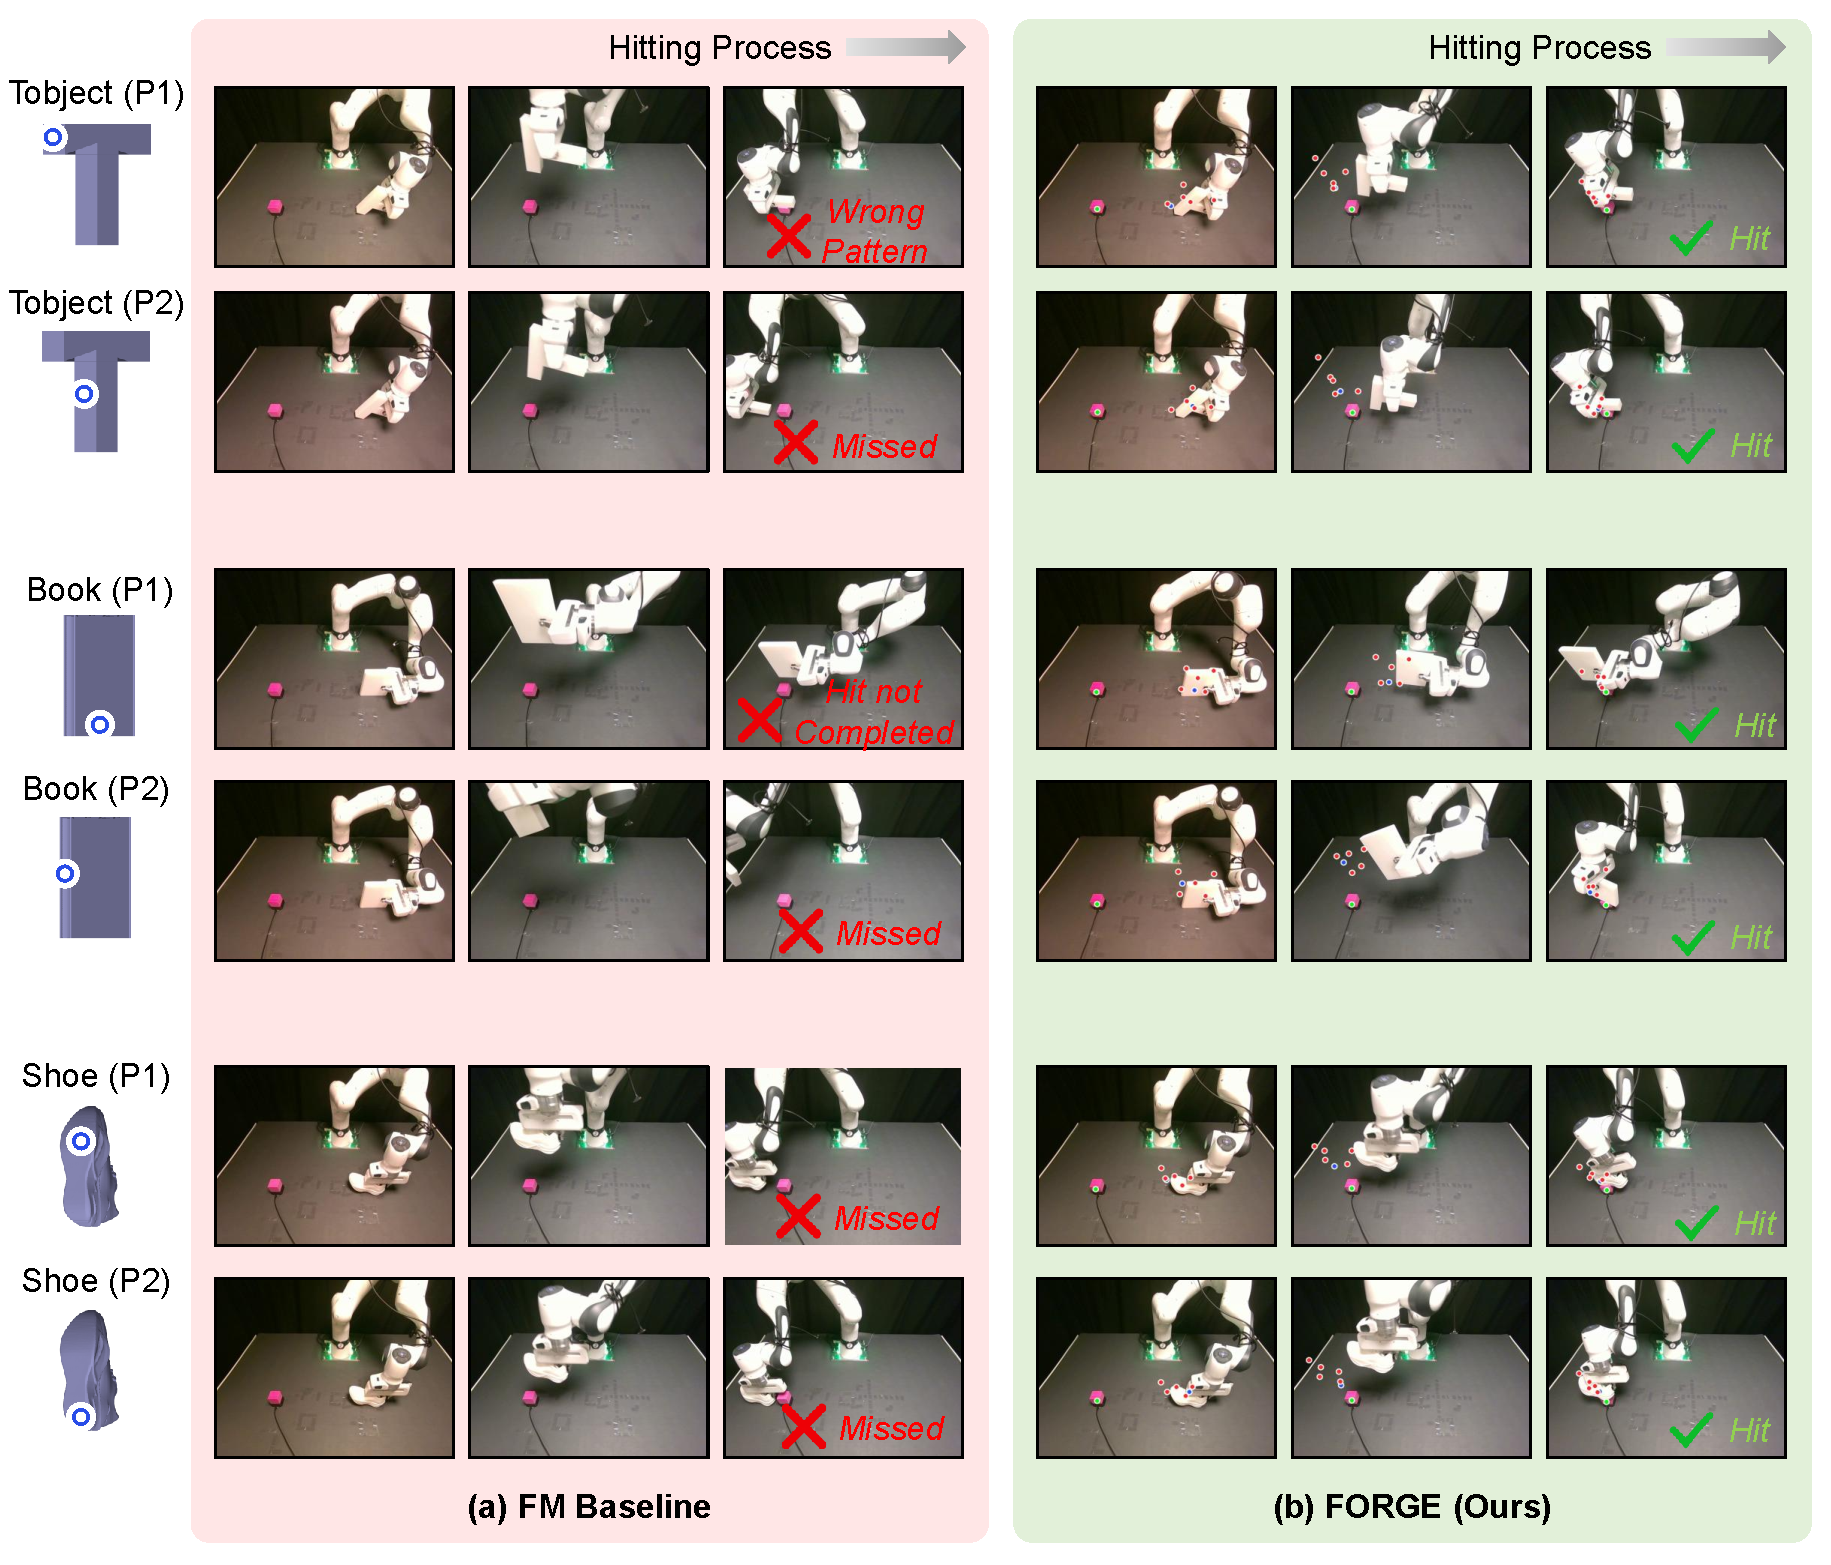
\includegraphics[width=1.0\linewidth]{figures/app-more-real-world.pdf}
    \caption{\textbf{Additional Real-World Qualitative Results.} (a) Failure cases of the FM baseline on unseen tools. (b) Successful demos of \algoname{} across hitting patterns. The blue point indicates the reference hitting point for each pattern.}
    \label{fig:app-more-real-world}
\end{figure}


\subsection{Training and Implementation Details}
\label{app:implementation_details}

All models are trained on NVIDIA RTX 6000 Pro GPUs. For all methods, we use an action chunk size of 8, a history horizon of 8, and a batch size of 64. We build the simulation benchmark on Robomimic and conduct real-world experiments on a Franka robot platform.

For baseline methods, we train each policy for 120,000 steps using the corresponding action-labeled data. For \algoname{}, we follow the two-stage training procedure described in Sec.~\ref{sec:FORGE}. We first pretrain the keypoint motion predictor $\pi_{\mathrm{sys2}}$ on action-free data from all tools for 240,000 steps. We then freeze the pretrained predictor and fine-tune the grounded execution policy $\pi_{\mathrm{sys1}}$ on the same action-labeled data used by the baselines for 120,000 steps.


\begin{table}[ht]
\centering
\caption{\textbf{Additional Real-World Results.}
Success rate (SR) on three unseen tools. Each tool is evaluated under two hitting patterns with 10 rollouts per pattern.}
\label{tab:more_real_world_results}
\resizebox{\linewidth}{!}{
\begin{tabular}{lcccccccccc}
\toprule
\multirow{2}{*}{Method} 
& \multicolumn{3}{c}{Tobject} 
& \multicolumn{3}{c}{Book} 
& \multicolumn{3}{c}{Shoe} 
& \multirow{2}{*}{Overall} \\
\cmidrule(lr){2-4} 
\cmidrule(lr){5-7} 
\cmidrule(lr){8-10}
& P01 & P02 & Avg.
& P01 & P02 & Avg.
& P01 & P02 & Avg.
& \\

\midrule
FM~\cite{lipmanflow} 
& 0.00 & 0.60 & \cellcolor{gray!15} 0.30
& 0.50 & 0.00 & \cellcolor{gray!15} 0.25
& 0.00 & 0.20 & \cellcolor{gray!15} 0.10
& \cellcolor{teal!10} 0.22 \\

\midrule
\algoname{} (Ours) 
& \textbf{0.60} & \textbf{0.80} & \cellcolor{gray!18}\textbf{0.70}
& \textbf{0.60} & \textbf{1.00} & \cellcolor{gray!18}\textbf{0.80}
& \textbf{0.20} & \textbf{0.60} & \cellcolor{gray!18}\textbf{0.40}
& \cellcolor{teal!10}\textbf{0.63} \\
\bottomrule
\end{tabular}
}
\end{table}

\begin{figure}[ht]
    \centering
    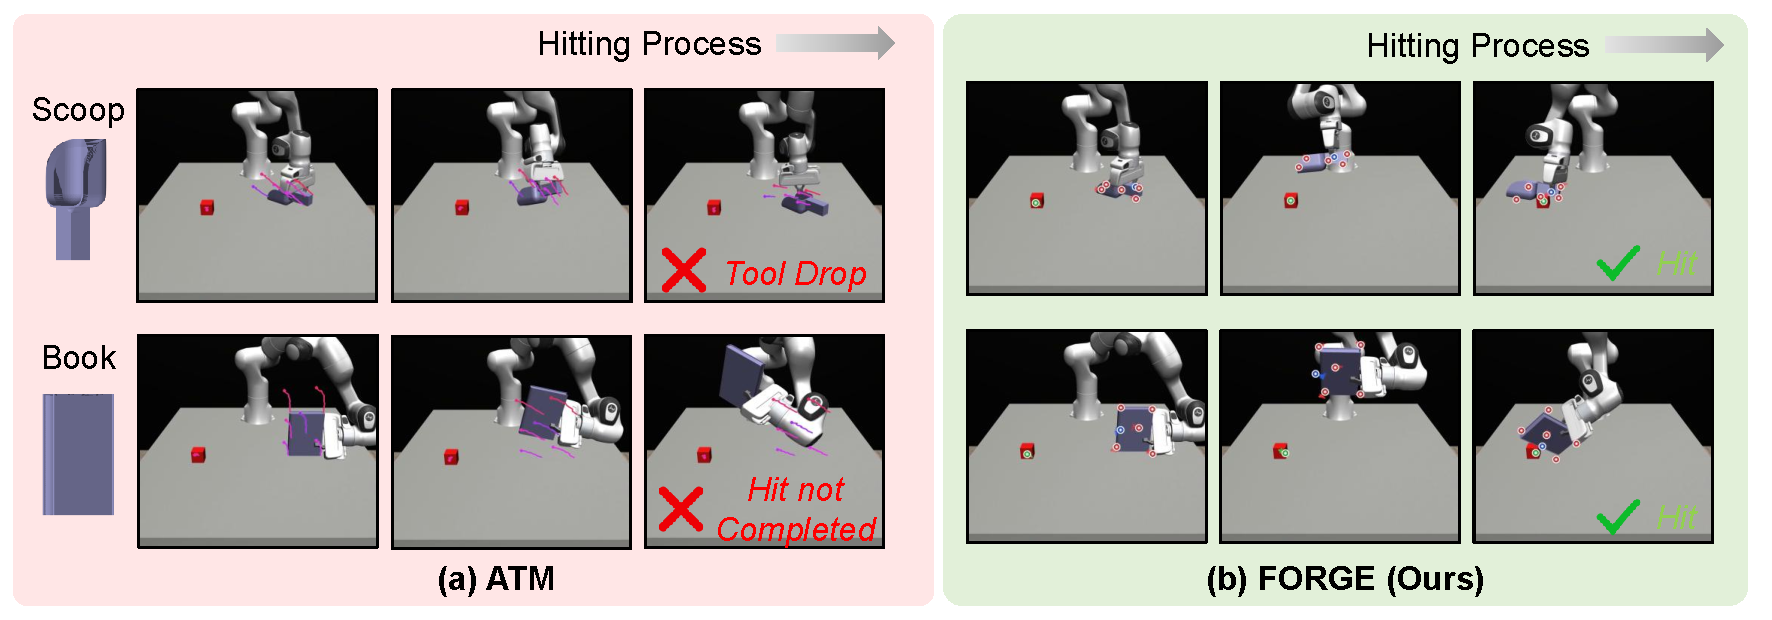
\includegraphics[width=1.0\linewidth]{figures/app-compared-with-ATM.pdf}
    \caption{\textbf{Additional Qualitative Comparison with ATM.}
    (a) Failure cases of ATM on unseen tools. (b) Successful demos of \algoname{} with predicted keypoint-based functional plans.}
    \label{fig:app-compare-atm}
\end{figure}


\section{Additional Experimental Results}
\label{app:additional_experimental_results}

In this section, we first present additional real-world experiments with diverse unseen tools and hitting patterns in Appx.~\ref{app:more_real_world_experiments}, and then provide more qualitative analysis in Appx.~\ref{app:more_qualitative_results}.

\subsection{More Real-World Experiments}
\label{app:more_real_world_experiments}
We conduct additional real-world experiments to evaluate \algoname{} under more diverse tool and hitting-pattern variations. Specifically, we train all methods on three seen tools, including hammer, pickaxe, and mustard, and evaluate them on three unseen tools: tobject, book, and shoe. Each unseen tool contains two hitting patterns, and each pattern is evaluated with 10 real-world rollout trials.

As shown in Tab.~\ref{tab:more_real_world_results}, \algoname{} outperforms the FM baseline across all three unseen tools, improving the overall success rate from 0.22 to 0.63. These results further confirm the main real-world finding: direct perception-to-action mapping struggles to adapt the hitting motion to novel tools, while keypoint-based functional plans provide explicit guidance for aligning the desired hitting region with the target.
The FM baseline mainly fails due to ineffective downward strikes, missed hits, or incorrect hitting patterns. Please refer to our supplementary videos for qualitative demonstrations.

% Please refer to our supplementary videos for qualitative demonstrations.

\subsection{Additional Qualitative Comparisons}
\label{app:more_qualitative_results}

\textbf{More Real-World Cases.}~~
Fig.~\ref{fig:app-more-real-world} provides additional real-world comparisons between the FM baseline and \algoname{} across different unseen tools and hitting patterns. The FM baseline exhibits three typical failure modes: ineffective downward strikes, missed hits, and incorrect hitting patterns. These failures show that an end-to-end policy cannot reliably infer which tool region should be used or how the motion should change for a novel tool. By contrast, \algoname{} uses predicted keypoint-based functional plans to guide contact-region alignment and motion execution, leading to successful hits across these cases. This further supports that functional generalization benefits from an explicit intermediate representation between perception and action. 

\textbf{Comparison with ATM.}~~
Fig.~\ref{fig:app-compare-atm} shows additional qualitative comparisons between ATM and \algoname{} on unseen tools. Although ATM also conditions the policy on keypoint trajectories, these trajectories are produced by a generic tracker and do not explicitly encode function-aware hitting motion. As a result, ATM often fails to guide the tool-specific contact region toward the target, leading to tool dropping or incomplete hits. In contrast, \algoname{} predicts function-aware keypoint trajectories that specify how the hitting point should approach the target before impact, enabling more reliable execution. These results further support our \textbf{H3} in Sec.~\ref{sec:experiments}: keypoint trajectories must encode functional motion intent rather than only generic point tracking.

Please refer to our supplementary videos for demos of both simulation and real-world experiments.



% \begin{table}[t]
% \centering
% \caption{Ablation study on the number of keypoints.}
% \label{tab:ablation_num_keypoints}
% \resizebox{0.5\linewidth}{!}{
% \begin{tabular}{lcccc}
% \toprule
% \# Keypoints & Scoop & Book & Shoe & Avg. \\
% \midrule
% 5 & 0.41 & 0.35 & 0.20 & 0.32 \\
% 7 & 0.42 & 0.42 & 0.23 & 0.36 \\
% 9 & 0.23 & 0.43 & 0.12 & 0.26 \\
% \bottomrule
% \end{tabular}
% }
% \end{table}


% \begin{table}[t]
% \centering
% \caption{\textbf{Ablation on Action-Labeled Tool Diversity.} Success rate (SR) of \algoname{} under different training-to-testing tool splits. `M-to-N' denotes training on $M$ tools and testing on $N$ unseen tools.}
% \resizebox{0.5\linewidth}{!}{
% \begin{tabular}{lcccc}
% \toprule
% Methods & Scoop & Book & Shoe & Avg. \\
% \midrule
% 1-to-3 & 0.17 & 0.10 & 0.14 & 0.14 \\
% 4-to-3 & 0.42 & 0.42 & 0.23 & 0.36 \\
% 7-to-3 & 0.40 & 0.58 & 0.28 & 0.42 \\
% \bottomrule
% \end{tabular}
% }
% \end{table}

% \begin{table}[ht]
% \centering
% \caption{\textbf{Ablation on Action-Labeled Tool Diversity.} Success rate (SR) of \algoname{} under different training-to-testing tool splits. `M-to-N' denotes training on $M$ tools and testing on $N$ unseen tools.}


% \label{tab:ablation_tool_generalization_setting}
% \resizebox{0.9\linewidth}{!}{
% \begin{tabular}{lcccccccc}
% \toprule
% \multirow{2}{*}{Method}
% & \multicolumn{8}{c}{Tools} \\
% \cmidrule(lr){2-9}
% & Hammer & Tobject & Pickaxe & Mustard & Scoop & Shoe & Book & Avg. \\
% \midrule
% \algoname{} (1-to-6) & -- & 0.26 & 0.34 & 0.17 & 0.14 & 0.10 & 0.23 & \cellcolor{teal!10} 0.21 \\
% \algoname{} (4-to-3) & -- & -- & -- & -- & 0.42 & 0.23 & 0.42 & \cellcolor{teal!10} 0.36 \\
% \algoname{} (6-to-1) & -- & -- & -- & -- & -- & -- & 0.52 & \cellcolor{teal!10} 0.52\\
% \bottomrule
% \end{tabular}
% }
% \end{table}



\end{document}
